\documentclass[12pt]{beamer}
\mode<presentation>
\usepackage[utf8]{inputenc}
\usepackage{graphicx}
\usepackage{amssymb,textcomp}
%\usepackage{beamerthemesplit}
\usepackage{beamerthemeBoadilla}
\usepackage{tikz}
\usetikzlibrary{decorations.pathreplacing}
\usepackage{booktabs}
\usepackage{amsmath}

\usefonttheme{serif}
\title{Unidad IV: Diferenciaci\'on e Integraci\'on Num\'erica}
\author{Prof. Jos\'e Luis Ram\'irez}
\date{\today}

\sloppy
\setlength{\emergencystretch}{3em} % Allow more flexibility in line breaking
\begin{document}

\maketitle

\begin{frame}
  \titlepage
\end{frame}

\begin{frame}{Contenido}
  \tableofcontents
\end{frame}

\section{Introducción}
\begin{frame}{Motivaci\'on}
  El flujo de calor en la interfaz suelo-aire puede calcularse con la ley de Faraday
  \begin{block}{}
    $$
    q = -k\rho C \frac{dT}{dz}
    $$
  \end{block}
  
  Donde $q =$ flujo de calor, $k =$ coeficiente de difusividad t\'ermica, $\rho =$ la densidad del suelo, $C =$ calor espec\'ifico del suelo.
\end{frame}
%%%%%%
\begin{frame}{Motivaci\'on}
  \begin{itemize}
    \item Las situaciones en las cuales se requiere el uso de la diferenciaci\'on num\'erica, ocurren cuando el conjunto de datos est\'a dado en la forma discreta y cuando la funci\'on que se va a derivar es complicada, por lo que la derivaci\'on anal\'itica es dif\'icil, cuando no imposible.
    \item<2-> Entonces, las soluciones num\'ericas son preferibles a las anal\'iticas, siempre que la funci\'on sea f\'acil de evaluar.
    \item<3-> Problemas que han sido estudiados, involucran en cierto modo el c\'alculo de la derivada de una funci\'on evaluada en un punto, como por ejemplo:
    \begin{enumerate}
      \item<4-> Interpolaci\'on C\'ubica de Trazador Sujeto.
      \item<5-> M\'etodo de Newton-Raphson.
      \item<6-> Ecuaciones Diferenciales.
    \end{enumerate}
  \end{itemize}
\end{frame}
%%%%%
\begin{frame}{Motivaci\'on}
    Hay distintas razones por la que la integraci\'on num\'erica se realiza.
    \begin{itemize}
    \item<2-> El integrando $f(x)$ puede ser conocido solamente en ciertos puntos, tales como: obtenidos por muestreo. Algunos sistemas encajados y otras aplicaciones inform\'aticas pueden necesitar la integraci\'on num\'erica por esta raz\'on.    
    \item<3-> Un f\'ormula para el integrando puede ser conocido, pero puede ser dif\'icil o imposible de encontrar su antiderivada. Un ejemplo de tal integrando es $f(x) = e^{-x^2}$, cuya antiderivada no se puede escribir en forma elemental.    
    \item<4-> Puede ser posible encontrar una antiderivada simb\'olicamente, pero puede ser m\'as f\'acil computar una aproximaci\'on num\'erica que computar la antiderivada. \'Ese puede ser el caso si la antiderivada se da como una serie o producto infinita, o si su evaluaci\'on requiere una funci\'on especial la cu\'al no est\'a disponible.
  \end{itemize}
\end{frame}
% %%%%%
\section{Diferenciaci\'on Num\'erica}
\begin{frame}{Diferenciaci\'on Num\'erica}
    \begin{itemize}
        \item<1-> La diferenciaci\'on num\'erica puede calcularse usando la definici\'on de derivada
        \begin{block}{}
          $$
          f'(x_0) = \lim_{h\rightarrow0}\frac{f(x_0+h)-f(x_0)}{h}
          $$
        \end{block}
        \item<2-> Tomando una $h$ peque\~na. Si $h > 0$ se llama f\'ormula de diferencia progresiva, si $h < 0$ se llama f\'ormula de diferencia regresiva.
    \end{itemize}
\end{frame}
%%%%%%
\begin{frame}{Diferenciaci\'on Num\'erica}
  \begin{itemize}
    \item Para calcular la aproximaci\'on num\'erica de la derivada en un punto, se puede generar una sucesi\'on $\{h_k\}$, tal que $h_k \to 0$ y se calcula el cociente
    \begin{block}{}
      $$
      D_k = \dfrac{f(x_0+h_k)-f(x_0)}{h_k} = \dfrac{f_k-f_0}{h_k}
      $$
    \end{block}
    \item<2-> Generando entonces una sucesi\'on $D_1, D_2, D_3,\ldots, D_n$ y tomando a $D_n$ como la aproximaci\'on deseada, el problema est\'a en conocer cual valor de $h_k$ garantiza una buena aproximaci\'on
    \item Si se toma un valor muy grande de $h_k$ la aproximaci\'on no es aceptable y si $h_k$ es muy peque\~no la diferencia $f(x + h_k) - f(x) \approx 0$ ocurre una p\'erdida de d\'igitos significativos
  \end{itemize}
\end{frame}
%%%%%
\begin{frame}{Diferenciaci\'on Num\'erica}
  \begin{itemize}
    \item La siguiente tabla muestra los cocientes $D_k$ para aproximar la derivada de $f(x) = \sin(x)$ en $x = 2$ cuyo valor con nueve cifras significativas es $f'(2) = -0.416146837$.
  \end{itemize}
  \begin{table}[!ht]
    \small
    \begin{center}
      \begin{tabular}{|c||c||c||c|}\hline
      $h_k$  & $f_k$ & $f_k-f$ & $\frac{f_k-f}{h_k}$ \\\hline\hline
    $10^{-1}$ & 0.8632093666 & -0.0460880602 & -0.4608806018\\
    $10^{-2}$ & 0.9050905633 & -0.0042068635 & -0.4206863500\\
    $10^{-3}$ & 0.9088808254 & -0.0004166014 & -0.4166014159\\
    $10^{-4}$ & 0.9092558076 & -0.0000416192 & -0.4161923007\\
    $10^{-5}$ & 0.9092932653 & -0.0000041615 & -0.4161513830\\
    $10^{-6}$ & 0.9092970107 & -0.0000004161 & -0.4161472913\\
    $10^{-7}$ & 0.9092973852 & -0.0000000416 & -0.4161468814\\
    $10^{-8}$ & 0.9092974227 & -0.0000000042 & -0.4161468392\\
    $10^{-9}$ & 0.9092974264 & -0.0000000004 & -0.4161468947\\
    $10^{-10}$& 0.9092974268 & -0.0000000000 & -0.4161471168\\\hline
    \end{tabular}
     \caption{Aproximaci\'on del $(\sin(2))'=cos(2)$.}
     \end{center}     
    \end{table}    
\end{frame}
%%%%%
\begin{frame}{Diferenciaci\'on Num\'erica}
  \begin{itemize}
    \item ?`Cu\'an buena es esta aproximaci\'on de la derivada? Por el Teorema de Taylor se sabe que:
    $$
    f(x_0+h) = f(x_0) + f'(x_0)h + \frac{f''(\xi_h)h^2}{2} 
    $$         
    donde $\xi_h$ est\'a entre $x_0$ y $x_0+h$.
    \item Despejando ahora a $f'(x_0)$ en esta f\'ormula se tiene que:
    $$
    f'(x_0) = \frac{f(x_0+h)-f(x_0)}{h} - \frac{hf''(\xi_h)}{2}
    $$
    \item Esta f\'ormula nos dice que se aproxima a $f'(x_0)$ con un error proporcional a $h$, es decir, $f'(x_0) \approx O(h)$.    
  \end{itemize}
\end{frame}
%%%%%
\begin{frame}{Diferenciaci\'on Num\'erica}
  \begin{block}{Ejemplo:}
    Tomando $f(x)=x^9$ se desea aproximar $f'(1)$ cuyo valor exacto es nueve. En la siguiente figura se ilustran los errores absolutos como funci\'on de $h$ en escala logar\'itmica. 
    \end{block}
\end{frame}
%%%%%
\begin{frame}{Diferenciaci\'on Num\'erica}
  \begin{center}
    \begin{figure}
      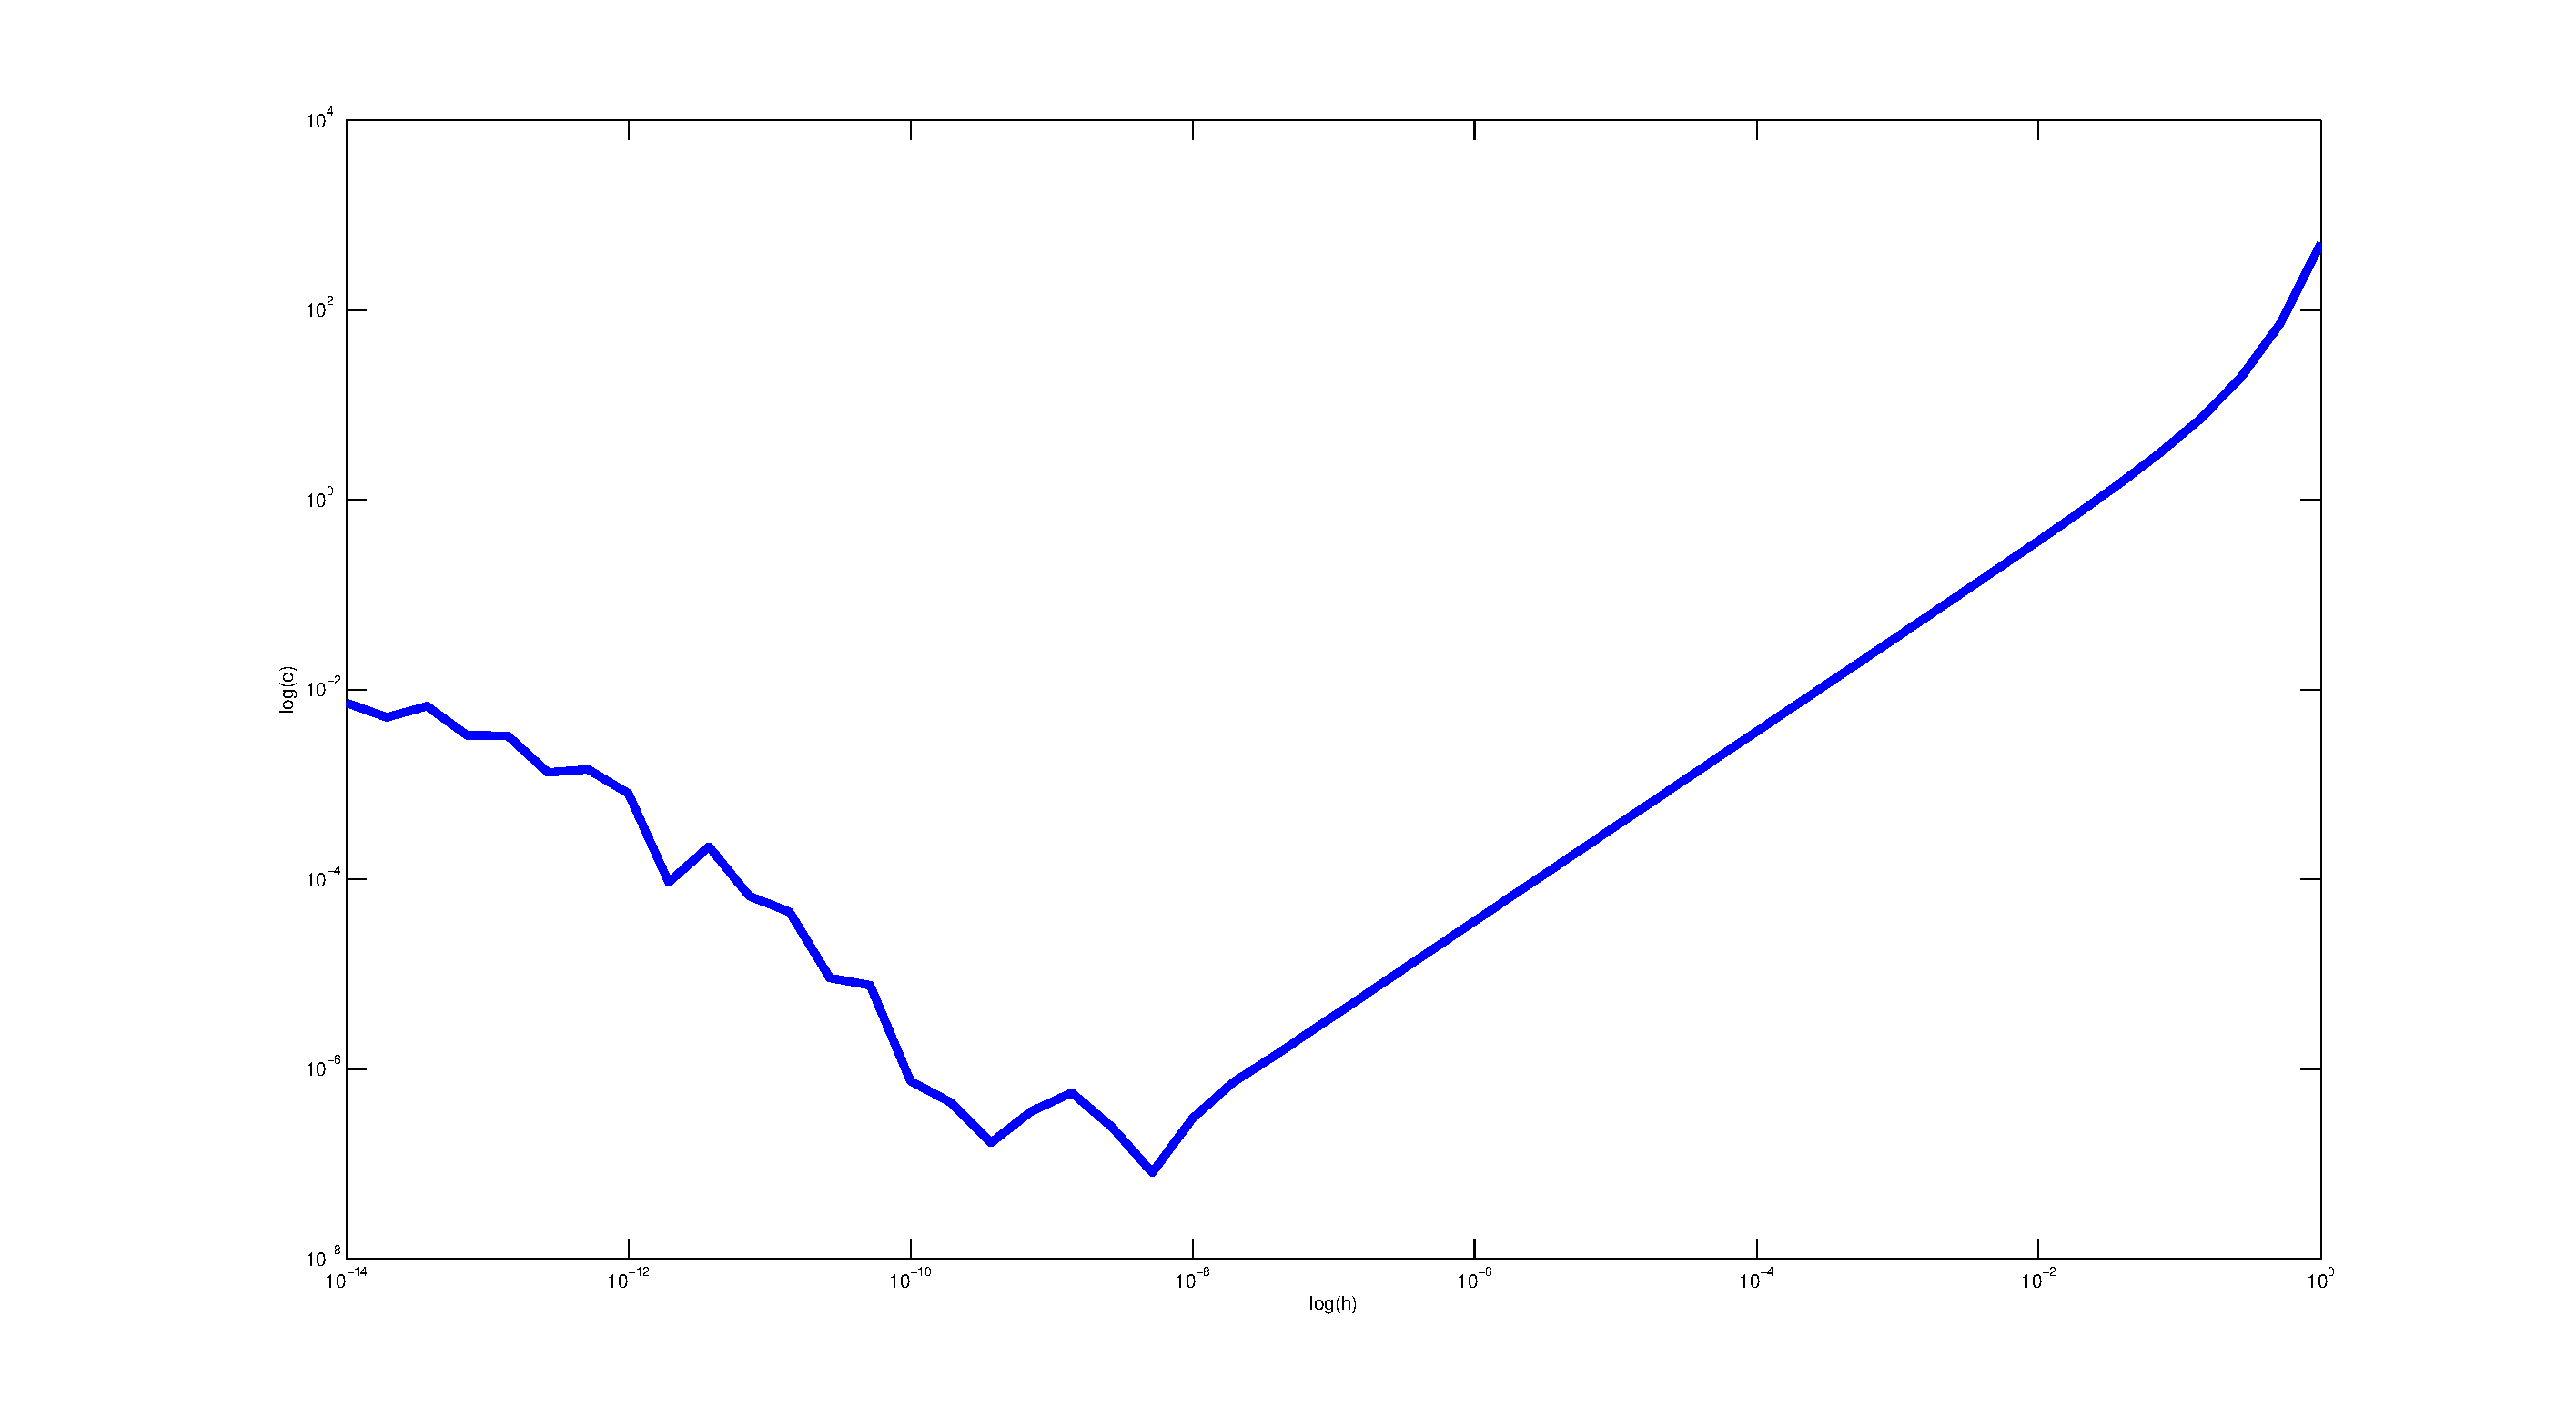
\includegraphics[scale=0.25]{ejem1.eps}
      \caption{Aproximaci\'on de $f'(1)$ para $f(x)=x^9$.}
    \end{figure}
  \end{center}
\end{frame}
%%%%%
\begin{frame}{Diferenciaci\'on Num\'erica}
  Se puede ver que los errores disminuyen hasta un cierto valor cr\'itico $h_{min}$ luego del cual los errores aumentan seg\'un la $h$ disminuye. \textquestiondown Contradice esto el resultado de arriba de $O(h)$ del error?
  \begin{itemize}
    \item<2-> El resultado anterior es sobre la convergencia si la aritm\'etica es exacta y se dice que es un resultado asint\'otico.
    \item<3-> La figura ilustra los efectos de redondeo debido a la aritm\'etica finita, los cuales se hacen significativos para $h$ peque\~no y pueden afectar cualquier f\'ormula num\'erica para aproximar la derivada.
  \end{itemize}
\end{frame}
%%%%%
\begin{frame}{Diferenciaci\'on Num\'erica}
  \begin{block}{Definici\'on:}
    El error de truncamiento se define como:
    $$
    E = |Du(x) - u'(x)|
    $$
    donde $u'(x)$ es la derivada y $Du(x)$ es su aproximaci\'on. Adem\'as, si $E \leq Ch^p$, se dice que el esquema $Du(x)$ tiene un orden de precisi\'on $p$, $O(h^p)$, siempre que $C$ sea una constante, la cual usualmente depende
    de la regularidad de $u(x)$.
  \end{block}
\end{frame}
%%%%%
\begin{frame}{Diferenciaci\'on Num\'erica}
  \begin{itemize}
    \item Una f\'ormula con un grado de aproximaci\'on digamos $O(h^2)$ es preferible a una de $O(h)$
    \item<2-> ya que los errores (te\'oricos) tienden a cero m\'as r\'apido y as\'i la $h$ no se tiene que hacerse tan peque\~na reduciendo as\'i los efectos de los errores por la aritm\'etica finita.
    \item<3-> Es posible, mejorar la precisi\'on de la siguiente manera: Sean los polinomios de Taylor de las funciones $f(x_0 + h)$ y $f(x_0 - h)$, suponiendo que la funci\'on es al menos tres veces derivable:
    \begin{align*}
    f(x_0+h) &= f(x_0) + f'(x_0)h + \dfrac{f''(x_0)}{2}h^2 + \dfrac{f'''(\xi_1)}{6}h^3\\
    f(x_0-h) &= f(x_0) - f'(x_0)h + \dfrac{f''(x_0)}{2}h^2 - \dfrac{f'''(\xi_2)}{6}h^3
    \end{align*}
  \end{itemize}
\end{frame}
%%%%%
\begin{frame}{Diferenciaci\'on Num\'erica}
  \begin{itemize}
    \item Restando ambas ecuaciones y resolviendo para $f'(x_0)$:
    $$
    f'(x_0) = \dfrac{f(x_0+h)-f(x_0-h)}{2h} - \dfrac{h^2}{12}(f'''(\xi_1)+f'''(\xi_2))
    $$
    \item<2-> Como $f \in \mathcal{C}^3 [x_0-h, x_0+h]$, entonces por el teorema del valor intermedio existe $\xi \in [x_0-h, x_0+h]$ tal que,
    $$
    f'''(\xi) = \dfrac{f'''(\xi_1)+f'''(\xi_2)}{2}
    $$   
  \end{itemize}
\end{frame}
%%%%%
\begin{frame}{Diferenciaci\'on Num\'erica}
  \begin{itemize}
    \item Por lo anterior queda entonces que:
    $$
    f'(x_0) = \dfrac{f(x_0+h)-f(x_0-h)}{2h} - \dfrac{f'''(\xi)}{6}h^2
    $$
    \item<2-> A esta expresi\'on se le llama f\'ormula de diferencia centrada, el orden de precisi\'on es 2, mientras que el error de truncamiento es $O(h^2)$.
    \end{itemize}
\end{frame}
%%%%
\begin{frame}{Diferenciaci\'on Num\'erica}
\begin{center}
 \begin{figure}
 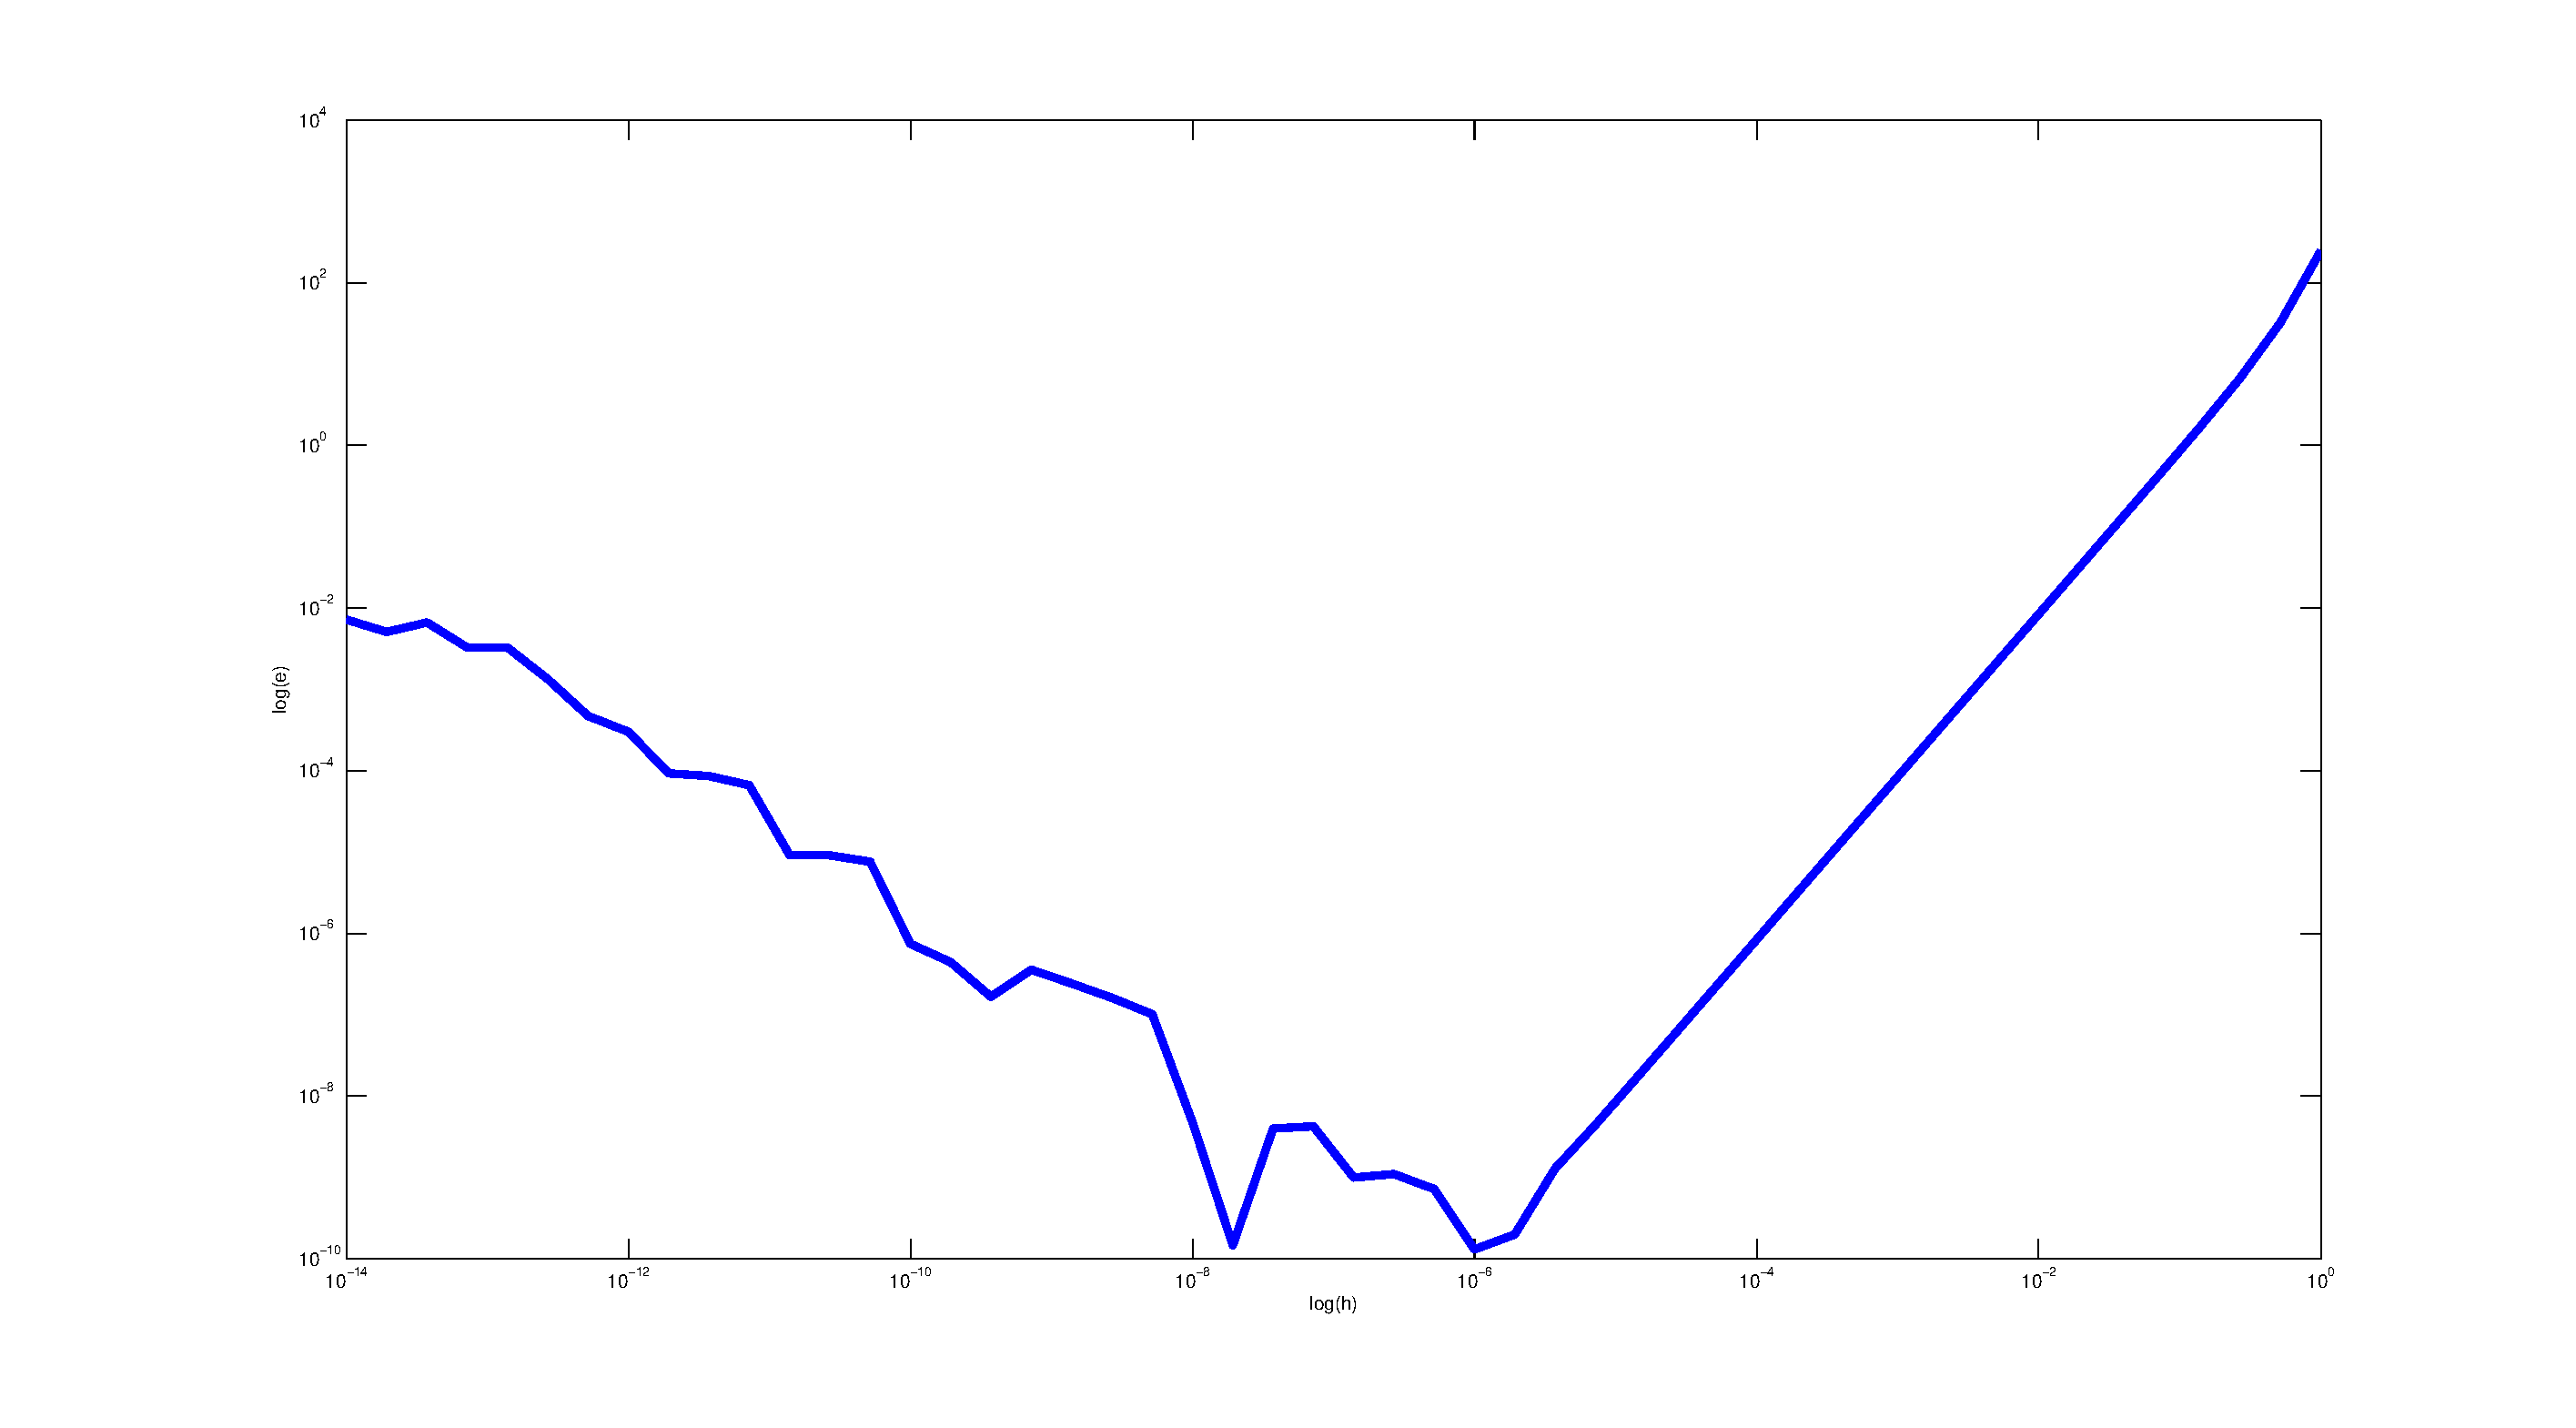
\includegraphics[scale=0.25]{ejem2.eps}
 \caption{Aproximaci\'on de $f'(1)$ para $f(x)=x^9$.}
\end{figure}
\end{center}
\end{frame}
%%%%%
\begin{frame}{F\'ormula de los $n$ puntos.}
El siguiente teorema utiliza el polinomio interpolador de una funci\'on $f$ para obtener f\'ormulas de aproximaci\'on a la derivada de una funci\'on $f$.
\uncover<2->{
\begin{block}{Teorema 1 (f\'ormula de $n$ puntos)}
Sea $f$ una funci\'on de clase $C^{n+1} [a, b]$ y $\{x_1,x_2,\ldots,x_n\}$ $n$ puntos distintos de dicho intervalo. Si llamamos $L_i(x)$ a los correspondientes polinomios elementales de Lagrange de grado $n-1$, entonces existe un punto $\xi \in [a,b]$ tal que
$$
f'(x_k) = \sum_{i=1}^nf(x_i)L'_i(x_k) + \frac{f^{(n)}(\xi)}{n!}\prod_{i=1,i\neq k}^n(x_k-x_i)
$$
\end{block}}
\end{frame}+
%%%%
\begin{frame}{F\'ormula de los $n$ puntos.}
  \begin{itemize}
    \item El polinomio de segundo grado que interpola a $f$ en los puntos $x_0,x_1,x_2$, tiene por polinomios elementales:
  \end{itemize}
\begin{align*}
\uncover<2->{L_0(x) = \frac{(x-x_1)(x-x_2)}{(x_0-x_1)(x_0-x_2)} & \Rightarrow L'_0(x) = \frac{(x-x_2)+(x-x_1)}{(x_0-x_1)(x_0-x_2)}\\}
\uncover<3->{L_1(x) = \frac{(x-x_0)(x-x_2)}{(x_1-x_0)(x_1-x_2)} & \Rightarrow L'_1(x) = \frac{(x-x_2)+(x-x_0)}{(x_1-x_0)(x_1-x_2)}\\}
\uncover<4->{L_2(x) = \frac{(x-x_0)(x-x_1)}{(x_2-x_0)(x_2-x_1)} & \Rightarrow L'_2(x) = \frac{(x-x_1)+(x-x_0)}{(x_2-x_0)(x_2-x_1)}}
\end{align*}
\end{frame}
%%%%
\begin{frame}{F\'ormula de los $n$ puntos}
  \begin{itemize}
    \item De esta manera, siguiendo el teorema anterior, se tendr\'ia que:
    {\footnotesize
      \begin{align*}
f'(x_k) &= \frac{f(x_0)[(x_k-x_2)+(x_k-x_1)]}{(x_0-x_1)(x_0-x_2)} + \frac{f(x_1)[(x_k-x_2)+(x_k-x_0)]}{(x_1-x_0)(x_1-x_2)}\\
 & + \frac{f(x_2)[(x_k-x_1)+(x_k-x_0)]}{(x_2-x_0)(x_2-x_1)} + \frac{f'''(\xi)}{3!}\prod_{i=0,i\neq k}^2(x_k-x_i)\\
& \qquad\qquad\qquad\qquad\qquad\qquad\qquad\qquad\qquad\forall k=0,1,2
\end{align*}}
    \end{itemize}
\end{frame}
%%%%
\begin{frame}{F\'ormula centrada de tres puntos.}
Si tomamos $x_0 = x_1-h$, $x_1 = x_1$ y $x_2 = x_1 + h$ para aproximar $f'(x_1)$, nos queda que:
\begin{align*}
f'(x_1) =&  \frac{f(x_0)(x_1-x_2)}{(x_0-x_1)(x_0-x_2)} + \frac{f(x_1)[(x_1-x_2)+(x_1-x_0)]}{(x_1-x_0)(x_1-x_2)}\\
 &+ \frac{f(x_2)(x_1-x_0)}{(x_2-x_0)(x_2-x_1)} + \frac{f'''(\xi)}{3!}\prod_{i=0,i\neq 1}^2(x_1-x_i)
\end{align*}
\uncover<2->{Sustituyendo $x_0$ y $x_2$, y simplificando la expresi\'on se obtiene:
\begin{align*}
f'(x_1) & = \frac{f(x_1+h)-f(x_1-h)}{2h} - \frac{f'''(\xi)}{6}h^2
\end{align*}}
\end{frame}
%%%%
\begin{frame}{F\'ormula progresiva de tres puntos.}
Si tomamos $x_0 = x_0$, $x_1 = x_0+h$ y $x_2 = x_0 + 2h$ para aproximar $f'(x_0)$ con $h > 0$ , queda que:
\begin{align*}
f'(x_0) &=  \frac{f(x_0)[(x_0-x_2)+(x_0-x_1)]}{(x_0-x_1)(x_0-x_2)} + \frac{f(x_1)(x_0-x_2)}{(x_1-x_0)(x_1-x_2)}\\
& + \frac{f(x_2)(x_0-x_1)}{(x_2-x_0)(x_2-x_1)} + \frac{f'''(\xi)}{3!}\prod_{i=0,i\neq 0}^2(x_0-x_i)
\end{align*}
\uncover<2->{Sustituyendo $x_1$ y $x_2$, y simplificando la expresi\'on se obtiene:
\begin{align*}
f'(x_0) & = \frac{-3f(x_0)+4f(x_0+h)-f(x_0+2h)}{2h} + \frac{f'''(\xi)}{3}h^2\nonumber
\end{align*}}
\end{frame}
%%%%
\begin{frame}{F\'ormula regresiva de tres puntos.}
Si tomamos $x_0 = x_2-2h$, $x_1 = x_2-h$ y $x_2 = x_2$ para aproximar $f'(x_2)$ con $h > 0$ , queda que:
\begin{align*}
f'(x_2) &=  \frac{f(x_0)(x_2-x_1)}{(x_0-x_1)(x_0-x_2)} + \frac{f(x_1)(x_2-x_0)}{(x_1-x_0)(x_1-x_2)}\\
 &+ \frac{f(x_2)[(x_2-x_1)+(x_2-x_0)]}{(x_2-x_0)(x_2-x_1)} + \frac{f'''(\xi)}{3!}\prod_{i=0,i\neq 2}^2(x_2-x_i)
\end{align*}
\uncover<2->{Sustituyendo $x_0$ y $x_1$, y simplificando la expresi\'on se obtiene:
\begin{align*}
f'(x_2) & = \frac{f(x_2-2h)-4f(x_2-h)+3f(x_2)}{2h} + \frac{f'''(\xi)}{3}h^2\nonumber
\end{align*}}
\end{frame}
%%%%
\begin{frame}{Derivadas de Orden Superior}
  \begin{itemize}
    \item A partir del desarrollo de Taylor de la funci\'on evaluada en $x_0 + h$ y $x_0 - h$, se puede
    obtener la f\'ormula para la que aproxima a la segunda derivada de la funci\'on $f$.
    \item<2-> Sea $0<|h|<\delta$ por Taylor, suponiendo que $f^{(4)}$ existe y es continua en $(x_0-\delta,x_0+\delta)$, $\xi_1$ entre $x_0$ y $x_0+h$, $\xi_2$ entre $x_0$ y $x_0-h$.
  \end{itemize}
  \uncover<3->{
  \begin{align*}
    f(x_0+h) &= f(x_0) + f'(x_0)h + \dfrac{f''(x_0)}{2}h^2 + \dfrac{f'''(x_0)}{6}h^3 + \dfrac{f^{(4)}(\xi_1)}{24}h^4\\
    f(x_0-h) &= f(x_0) - f'(x_0)h + \dfrac{f''(x_0)}{2}h^2 - \dfrac{f'''(x_0)}{6}h^3 + \dfrac{f^{(4)}(\xi_2)}{24}h^4
  \end{align*}}
\end{frame}
%%%%
\begin{frame}{Derivadas de Orden Superior}
  \begin{itemize}
    \item Sumandos ambas ecuaciones:
    {\small
    $$
     f(x_0+h) + f(x_0-h) = 2f(x_0) +2\dfrac{f''(x_0)}{2}h^2 + \dfrac{h^4}{24}\left(f^{(4)}(\xi_1)+f^{(4)}(\xi_2)\right)
     $$}
     \item y despejando $f''(x_0)$ de esta expresi\'on se obtiene:     
     $$
     f''(x_0) = \dfrac{f(x_0+h) - 2f(x_0) + f(x_0-h)}{h^2} + \dfrac{f^{(4)}(\xi)}{12}h^2 
    $$
    con $\xi \in (x_0-h,x_0+h)$
  \end{itemize}
\end{frame}
%%%%%
\subsection{Extrapolaci\'on de Richardson}
\begin{frame}{Extrapolaci\'on de Richardson}
  \begin{itemize}
    \item El proceso de obtener una estimaci\'on mejorada para el valor de Integrales, Derivadas, Ecuaciones Diferenciales, etc., con base
    en dos o m\'as aplicaciones de una f\'ormula, empleando diferentes longitudes de intervalo, se denomina Extrapolaci\'on.
    \item<2-> Uno de los m\'os conocidos es el de Extrapolaci\'on de Richardson o Aproximaci\'on diferida al l\'imite.
    \item<3-> Supongase que $G(h)$ es una expresi\'on que aproxima a una cantidad $G$
    \item<4-> entonces se tiene que $G - G(h) = E_T$ , donde $E_T$ es
    el error de truncamiento que se comete al aproximar a $G$ por $G(h)$.
  \end{itemize}
\end{frame}
%%%%%
\begin{frame}{Extrapolaci\'on de Richardson}
  \begin{itemize}
    \item<1-> Suponiendo:
    $$
    E_T = c_1 h + c_2 h^2 + c_3 h^3 + c_4 h^4 + \cdots,
    $$
    luego
    $$
     G = G(h) + c_1 h + c_2 h^2 + c_3 h^3 + c_4 h^4 + \cdots \qquad h>0
    $$
    \item<2-> Tomando $h=\dfrac{h}{2}$, entonces
    $$
    G = G\left(\dfrac{h}{2}\right) + c_1 \dfrac{h}{2} + c_2 \dfrac{h^2}{4} + c_3 \dfrac{h^3}{8} + c_4 \dfrac{h^4}{16} + \cdots
    \qquad h>0 
    $$
  \end{itemize}
\end{frame}
%%%%%
\begin{frame}{Extrapolaci\'on de Richardson}
  \begin{itemize}
    \item<1-> Si se multiplica por 2 a la \'ultima ecuaci\'ony se le resta $G$, entonces
    \small{
    $$
    2G-G = 2G\left(\dfrac{h}{2}\right)+ c_1 h + c_2 \dfrac{h^2}{2} + c_3\dfrac{h^3}{4} + \cdots
    - G(h) - c_1 h - c_2 h^2 - c_3 h^3 - \cdots 
    $$}
    \item<2-> o sea que:
    $$
    G = 2G\left(\dfrac{h}{2}\right)- G(h)- c_2 \dfrac{h^2}{2} - c_3 \dfrac{3h^3}{4} - c_4\dfrac{7h^4}{8} - \cdots
    $$
    \item<3-> luego
    $$
    G = \left[G\left(\dfrac{h}{2}\right)+\left(G\left(\dfrac{h}{2}\right)-G(h)\right)\right]- c_2 \dfrac{h^2}{2} - c_3 
    \dfrac{3h^3}{4} - c_4\dfrac{7h^4}{8} - \cdots
    $$
  \end{itemize}
\end{frame}
%%%%%
\begin{frame}{Extrapolaci\'on de Richardson}
  \begin{itemize}
    \item Para simplificar los c\'alculos denotese $G(h) \equiv G_1(h)$, la expresi\'on para $O(h^2)$, es entonces
    $$
    G = G_2(h) - c_2 \dfrac{h^2}{2} - c_3\dfrac{3h^3}{4} - c_4\dfrac{7h^4}{8} - \cdots
    $$
    donde $G_2(h) = G_1\left(\dfrac{h}{2}\right)+\left(G_1\left(\dfrac{h}{2}\right)-G_1(h)\right)$
  \end{itemize}  
\end{frame}
%%%%%
\begin{frame}{Extrapolaci\'on de Richardson}
  \begin{itemize}
    \item Al igual que antes reemplazamos  $h$ por $\dfrac{h}{2}$, se tiene que
    $$
     G = G_2\left(\dfrac{h}{2}\right) - c_2 \dfrac{h^2}{8} - c_3\dfrac{3h^3}{32} - c_4\dfrac{7h^4}{128} - \cdots
    $$
    \item<2-> Restando cuatro veces esta ecuaci\'on a la original se obtiene:
    $$
    4G-G = 4G_2\left(\dfrac{h}{2}\right) -G_2(h)- c_2 \dfrac{h^2}{2} - c_3\dfrac{3h^3}{8} - \cdots + 
    c_2 \dfrac{h^2}{2} + c_3\dfrac{3h^3}{4} + \cdots
    $$  
    \item<3-> o sea que
    $$
    3G = 4G_2\left(\dfrac{h}{2}\right) -G_2(h)+ c_3\dfrac{3h^3}{8} + c_4\dfrac{21h^4}{32} + \cdots
    $$
  \end{itemize}
\end{frame}
%%%%%
\begin{frame}{Extrapolaci\'on de Richardson}
  \begin{itemize}
    \item luego
    $$
    G = \left[G_2\left(\dfrac{h}{2}\right)+\dfrac{G_2\left(\dfrac{h}{2}\right)-G_2(h)}{3}\right]+ c_3\dfrac{h^3}{8} + 
    c_4\dfrac{7h^4}{32} + \cdots
    $$
    \item<2-> Denotando
    $$
    G_3(h) = G_2\left(\dfrac{h}{2}\right)+\dfrac{G_2\left(\dfrac{h}{2}\right)-G_2(h)}{3}
    $$
    se tiene la expresi\'on para $O(h^3)$ dada por    
    $$
     G = G_3(h) + c_3\dfrac{h^3}{8} + c_4\dfrac{7h^4}{32} + \cdots
    $$
  \end{itemize}
\end{frame}
%%%%%
\begin{frame}{Extrapolaci\'on de Richardson}
  \begin{itemize}
    \item reemplazando $h$ por $\dfrac{h}{2}$, se tiene que
    $$
      G = G_3\left(\dfrac{h}{2}\right) + \dfrac{h^3}{64}c_3 + \dfrac{7h^4}{512}c_4 + \cdots
    $$
    \item<2-> Restando ocho veces esta ecuaci\'on a la ecuaci\'on original se tiene que 
    $$
    7G = 8G_3\left(\dfrac{h}{2}\right) -G_3(h)- c_4\dfrac{7h^4}{64} - \cdots 
    $$
    \item<3-> o sea que
    $$
    7G = 7G_3\left(\dfrac{h}{2}\right)+G_3\left(\dfrac{h}{2}\right) -G_3(h)- c_4\dfrac{7h^4}{64} - \cdots 
    $$    
  \end{itemize}
\end{frame}
%%%%%
\begin{frame}{Extrapolaci\'on de Richardson}
  \begin{itemize}
    \item Por lo tanto
    $$
    G=\left[G_3\left(\dfrac{h}{2}\right)+\dfrac{G_3\left(\dfrac{h}{2}\right)-G_3(h)}{7}\right] - c_4\dfrac{7h^4}{64} - 
    \cdots
    $$
    \item<2-> As\'i que 
      $$
      G_4(h) = G_3\left(\dfrac{h}{2}\right)+\dfrac{G_3\left(\dfrac{h}{2}\right)-G_3(h)}{7}
      $$
      genera una aproximaci\'on $O(h^4)$ dada por
      $$
      G = G_4(h)- c_4\dfrac{7h^4}{64} - \cdots
      $$
  \end{itemize}
\end{frame}
%%%%%
\begin{frame}{Extrapolaci\'on de Richardson}
  \begin{itemize}
    \item Continuando con este proceso, la aproximaci\'on $O(h^n)$ es
    $$
    G = \left[G_{n-1}\left(\dfrac{h}{2}\right)+ \dfrac{G_{n-1}\left(\dfrac{h}{2}\right)-G_{n-1}(h)}{2^{n-1}-1}\right] + 
    \sum_{j=1}^{n-1}c_jh^j + O(h^n)
    $$
    \item<2-> donde
    $$
    G = G_n(h) + \sum_{j=1}^{n-1}c_jh^j + O(h^n)
    $$
    siendo
    $$
    G_n(h) = \left[G_{n-1}\left(\dfrac{h}{2}\right)+ \dfrac{G_{n-1}\left(\dfrac{h}{2}\right)-G_{n-1}(h)}{2^{n-1}-1}\right]
    $$    
  \end{itemize}
\end{frame}
%%%%&
\begin{frame}{Extrapolaci\'on de Richardson}
  \begin{itemize}
    \item La siguiente tabla muestra el uso de la Extrapolaci\'on de Richardson obtener una aproximaci\'on de orden 5, empleando 5 aproximaciones de orden 1
  \end{itemize}
    \begin{table}            
      \begin{center}
        \begin{tabular}{||l|llll||}\hline
          $O(h)$ & $O(h^2)$ & $O(h^3)$ & $O(h^4)$ & $O(h^5)$ \\\hline
          $G_1(h)$ &&&&\\
          $G_1(h/2)$ & $G_2(h)$ &&&\\
          $G_1(h/4)$ & $G_2(h/2)$ & $G_3(h)$ &&\\
          $G_1(h/8)$ & $G_2(h/4)$ & $G_3(h/2)$ & $G_4(h)$ &\\
          $G_1(h/16)$ & $G_2(h/8)$ & $G_3(h/4)$ & $G_4(h/2)$ & $G_5(h)$ \\\hline
          $\uparrow$ {\color{red}Medidas} & \multicolumn{1}{c}{$\uparrow$} & \multicolumn{2}{c}{\color{red}Extrapolaciones} & \multicolumn{1}{c||}{$\uparrow$} \\\hline
        \end{tabular}
      \end{center}
    \end{table}
\end{frame}
%%%%%
\frame
{
\frametitle{Extrapolaci\'on de Richardson. F\'ormula de tres puntos}
\begin{itemize}
\item Con este procedimiento se busca mejorar las ecuaciones obtenidas anteriormente para conseguir m\'as precisi\'on en la estimaci\'on de la derivada de $f$ en un punto $x$.
\item<2-> Supongase que $f(x)$ es de clase $C^n$ en $[x, x + h]$. En tal caso, su desarrollo en serie de Taylor alrededor de $x$ para los puntos $x + h$ y $x - h$ ser\'a de la forma
\begin{eqnarray}
 f(x+h) &=& \sum_{k=0}^\infty\frac{h^k}{k!}f^{(k)}(x)\nonumber\\
 f(x-h) &=& \sum_{k=0}^\infty\frac{(-1)^kh^k}{k!}f^{(k)}(x)\nonumber
\end{eqnarray}
\end{itemize}
}
%%%%
\frame
{
  \frametitle{Extrapolaci\'on de Richardson. F\'ormula de tres puntos}
  \begin{itemize}
    \item Restando ambas ecuaciones, todos los t\'erminos de orden par se cancelan, resultando
    $$
    f(x+h)-f(x-h) = 2hf'(x) + \frac{2}{3!}h^3f'''(x) + \frac{2}{5!}h^5f^{(5)}(x) + \cdots
    $$
    de donde, despejando $f'(x)$,
    $$
    f'(x) = \frac{f(x+h)-f(x-h)}{2h} - \left[\frac{1}{3!}h^2f^{(3)}(x)+\frac{1}{5!}h^4f^{(5)}(x)+\cdots\right]
    $$
  \end{itemize}
}
%%%%
\frame{
  \frametitle{Extrapolaci\'on de Richardson. F\'ormula de tres puntos}
  \begin{itemize}
    \item Lo que se puede escribir como:
    $$
    G = G_1(h) + a_2 h^2 + a_4 h^4 + a_6 h^6 + \cdots
    $$
    en la que $G = f'(x)$, la funci\'on $G_1(h)$ se define como $\frac{f(x+h)-f(x-h)}{2h}$  y $a_k = \frac{-1}{(k+1)!}f^{(k+1)}(x)$.
    \item<2-> Dado que $G_1(h)$ es el valor para la derivada, el error depende de t\'erminos en potencias de $h$, siendo el t\'ermino dominante el correspondiente a $h^2$.
  \end{itemize}
  }
  %%%%
  \frame{
    \frametitle{Extrapolaci\'on de Richardson. F\'ormula de tres puntos}
    \begin{itemize}
     \item<1-> Usando el m\'etodo de Richardson para conseguir que el t\'ermino dominante del error sea a\'un m\'as peque\~no. Escribiendo la ecuaci\'on evalu\'andola en $h/2$, lo que da:
    $$
    G = G_1\left(\frac{h}{2}\right) + a_2\frac{h^2}{4} + a_4\frac{h^4}{16} + a_6\frac{h^6}{64}+\cdots
    $$
    \item<2-> Restando esta ecuaci\'on multiplicada por 4 a la ecuaci\'on original, queda:
    $$
    3G = 4G_1\left(\frac{h}{2}\right) - G_1(h) - 3a_4\frac{h^4}{4} - 15a_6\frac{h^6}{16}-\cdots
    $$
    \item<3-> despejando la derivada $G$ queda como:
      $$
      G = \frac{4G_1\left(\frac{h}{2}\right)-G_1(h)}{3} - a_4\frac{h^4}{4} - 5a_6\frac{h^6}{16}-\cdots
    $$
  \end{itemize}
}
%%%%
\frame
{
  \frametitle{Extrapolaci\'on de Richardson. F\'ormula de tres puntos}
  \begin{itemize}
    \item Usando una simple combinaci\'on de $G_1(h)$ y $G_1(h/2)$, se obtiene una precisi\'on del orden de $h^4$, frente al orden $h^2$ que presenta $G_1(h)$.
    \item<2-> An\'alogamente se puede repetir el proceso tantas veces como se quiera; el siguente paso definir $G_2(h)=\frac{4G_1\left(\frac{h}{2}\right)-G_1(h)}{3}$ con lo que la ecuaci\'on evaluada en $h$ y en $h/2$ queda
    \begin{eqnarray}
    G &=& G_2(h) + b_4h^4 + b_6h^6 + \cdots\nonumber\\
    G &=& G_2\left(\frac{h}{2}\right) + b_4\frac{h^4}{16} + b_6\frac{h^6}{64} + \cdots\nonumber
    \end{eqnarray}
\end{itemize}
}
%%%%
\frame
{
  \frametitle{Extrapolaci\'on de Richardson. F\'ormula de tres puntos}
  \begin{itemize}
    \item Se puede despejar $G$, multiplicando la segunda ecuaci\'on por 16 y rest\'andole la primera:
    $$
    L = \frac{16G_2\left(\frac{h}{2}\right)-G(h)}{15} - b_6\frac{h^6}{20} -\cdots
    $$
    que es una estimaci\'on de $f'(x)$ con precisi\'on de orden $h^6$.
  \end{itemize}
}
%%%%
\frame
{
\frametitle{Generalizaci\'on}
\begin{itemize}
\item Si denotamos $G_k(h)$ una aproximaci\'on de orden $O(h^{2k})$ a $f'(x)$ entonces se tendr\'ia:
$$
f'(x) = G_k(h) + c_1h^{2k} + c_2h^{2k+2} + \cdots,\text{ para }k = 1,2,3,\ldots
$$
\item<2-> Considerando ahora $h/2$ en lugar de $h$ se tiene:
$$
f'(x) = G_k\left(\frac{h}{2}\right) + \frac{c_1}{4^k}h^{2k} + \frac{c_2}{4^{k+1}}h^{2k+2} + \cdots
$$
\item<3-> Multiplicando esta \'ultima ecuaci\'on por $4^k$ y restando la ecuaci\'on inicial resulta:
$$
f'(x) = \frac{4^kG_k(h/2) - G_k(h)}{4^k-1} + O(h^{2k+2})
$$
\end{itemize}
}
%%%%
\frame
{
  \frametitle{Generalizaci\'on}
  \begin{itemize}
    \item Por tanto, si denotamos 
    $$
    G_{k+1} = \frac{4^kG_k(h/2)-G_k(h)}{4^k-1}
    $$
    \item<2->entonces se tiene que se cumple:
    $$
    f'(x) = D_{k+1}(h) + O(h^{2k+2})
    $$
  \end{itemize}
}
%%%%
\frame
{
\frametitle{Ejemplo}
\begin{itemize}
  \item La f\'ormula en diferencias centrada para aproximar $f'(x_0)$ viene dada por:
  {\small
  $$
  f'(x_0) = \underbrace{\dfrac{f(x+h)-f(x-h)}{2h}}_{G_1(h)}-\underbrace{\dfrac{h^2}{6}f'''(\xi)+O(h^4)}_{\text{termino del error}}  
  $$}
  \item<2-> Con el objetivo de generar una f\'ormula que elimine el t\'ermino cuadr\'atico
  {\small
  $$
  G_2(h) = G_1\left(\frac{h}{2}\right) + \dfrac{G_1\left(\frac{h}{2}\right)-G_1(h)}{3}  
  $$
  \begin{align*}
    G_2(2h) & = \frac{f(x+h)-f(x-h)}{2h}+\dfrac{\frac{f(x+h)-f(x-h)}{2h}-\frac{f(x+2h)-f(x-2h)}{4h}}{3}\\
    & = \frac{8f(x+h)-8f(x-h)}{12h}+\frac{f(x+2h)-f(x-2h)}{12h}\\
    & = \frac{1}{12h}\left[f(x-2h)-8f(x-h)+8f(x+h)-f(x+2h)\right]  
  \end{align*}}
\end{itemize}
}  
%%%%%
\section{Integraci\'on Num\'erica}
\begin{frame}{Integraci\'on Num\'erica}
    \begin{itemize}
        \item Dada una funci\'on $f$ definida sobre un intervalo $[a,b]$, se desea calcular
        $$
        I(f) = \int_a^bf(x)dx
        $$
        \item<2-> La cuadratura o integraci\'on num\'erica consiste en obtener f\'ormulas aproximadas para calcular la integral $I(f)$ de $f$.
        \item<3->Estos m\'etodos son de gran utilidad cuando la integral no se puede calcular por m\'etodos anal\'iticos.        
    \end{itemize}
\end{frame}
%%%%%
\begin{frame}{Integraci\'on v\'ia Interpolaci\'on Polinomial}
  \begin{itemize}
    \item Una estrategia \'util para calcular el valor num\'erico de la integral dada consiste en reemplazar $f$ por otra funci\'on $g$, f\'acil de integrar, que aproxima a $f$ de forma adecuada.
    \item<2->Si $f \approx g$, se deduce que:
    $$
    \int_a^bf(x)dx \approx \int_a^bg(x)dx
    $$
    \item<3-> Los polinomios son buenos candidatos para el papel de $g$. De hecho, $g$ puede ser un polinomio que interpola a $f$ en cierto conjunto de nodos.    
  \end{itemize}
\end{frame}
%%%%%
\begin{frame}{Integraci\'on v\'ia Interpolaci\'on Polinomial}
  \begin{itemize}
    \item Sup\'ongase que se desea calcular la integral $I(f)$. Dado una serie de nodos, $x_0,x_1,\ldots,x_n$ en el intervalo
    $[a,b]$ se inicia un proceso de interpolaci\'on de Lagrange.
    \item<2-> El polinomio de grado menor o igual a $n$ que interpola a
    $f$ en los nodos es:
    $$
    p(x)=\sum_{i=0}^nf(x_i)L_i(x)
    $$
    \item<3-> La integral se puede escribir entonces como:
    $$
    \int_a^bf(x)dx \approx \int_a^bp(x)dx =   \sum_{i=0}^n\int_a^bf(x_i)L_i(x)dx
    $$    
  \end{itemize}
\end{frame} 
%%%%%
\begin{frame}{Integraci\'on v\'ia Interpolaci\'on Polinomial}
  \begin{itemize}
    \item Es decir, tenemos una f\'ormula general que se puede emplear para cualquier $f$ y que tiene la forma:
    $$
    \int_a^bf(x)dx \approx \sum_{i=0}^nA_if(x_i)
    $$    
    en donde
    $$
    A_i=\int_a^bL_i(x)dx
    $$
    \end{itemize}
\end{frame}
%%%%%
\subsection{Regla del Trapecio}
\begin{frame}{Regla del Trapecio}
  \begin{itemize}
    \item Empleando un polinomio de grado $n = 1$ y tomamos como nodos $x_0 = a$ y $x_1 = b$, se tiene el caso m\'as sencillo posible, en donde los polinomios de interpolaci\'on son:
    \begin{eqnarray}
     L_0(x) & = & \frac{b-x}{b-a}\nonumber\\
     L_1(x) & = & \frac{x-a}{b-a}\nonumber
    \end{eqnarray}
    \item<2-> por lo que:
    $$
    A_0 = \int_a^bL_0(x)dx = \frac{b-a}{2} = \int_a^bL_1(x)dx = A_1
    $$    
  \end{itemize}
\end{frame}
%%%%%
\begin{frame}{Regla del Trapecio}
  \begin{itemize}
    \item La f\'ormula de cuadratura correspondiente, tomando $h=b-a$, es:
    $$
    \int_a^bf(x)dx \approx \frac{b-a}{2}[f(a)+f(b)] = \dfrac{h}{2}\left(f(a)+f(b)\right)
    $$    
    \begin{center}
     \begin{figure}
     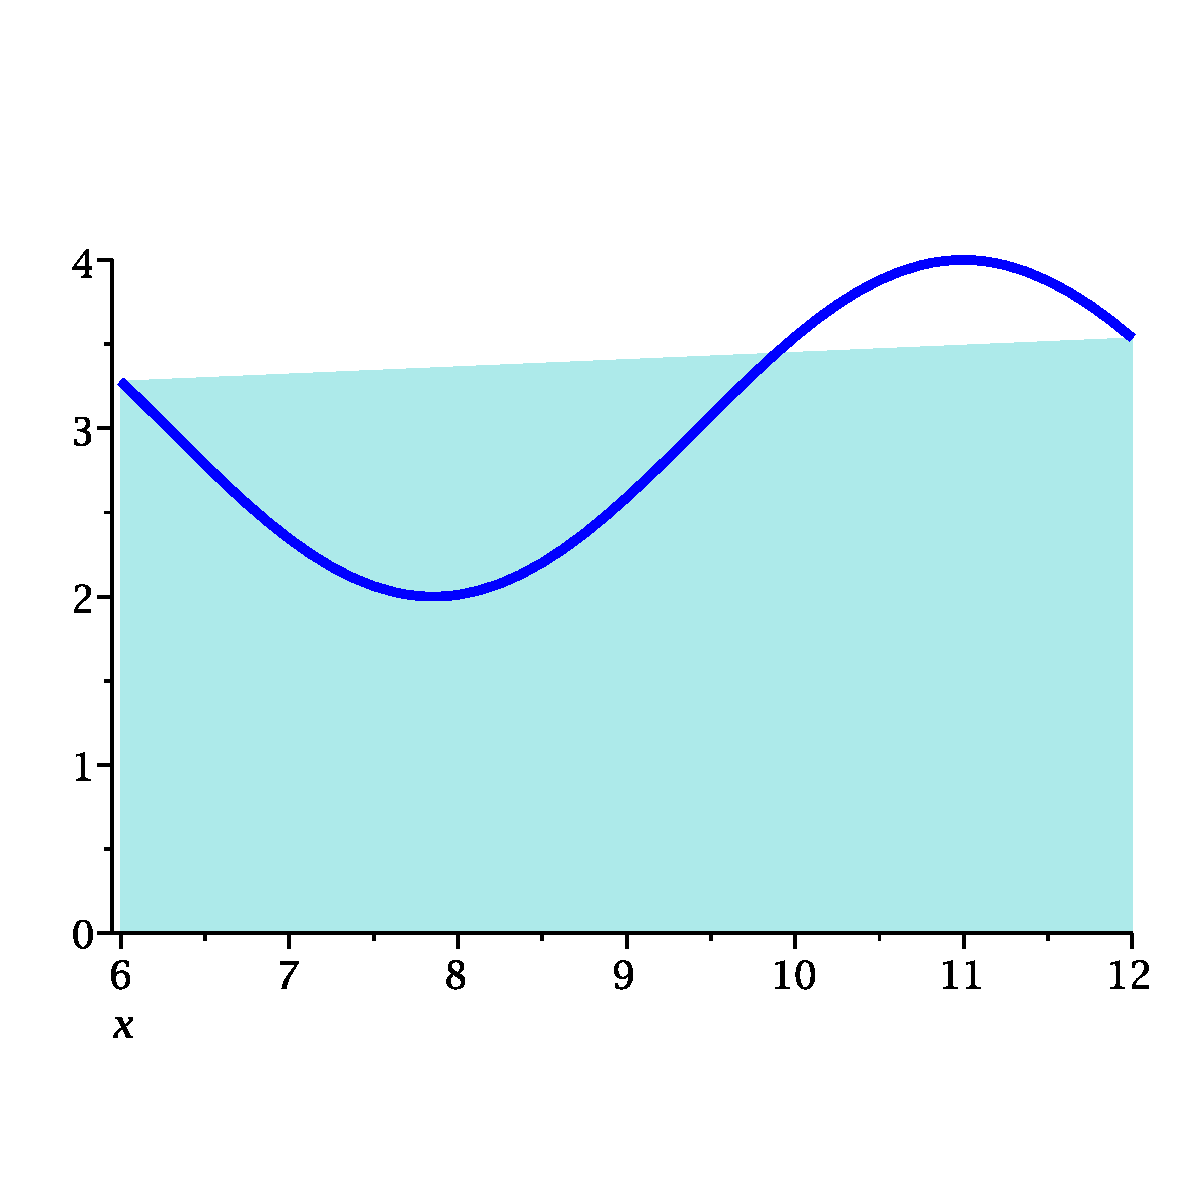
\includegraphics[scale=0.25]{trapz.eps}
    \end{figure}
    \end{center}
  \end{itemize}
\end{frame}
%%%%%
\begin{frame}{Regla del Trapecio}
  \begin{itemize}
    \item Se tiene entonces que:
    $$
    I = \int_a^bf(x)dx = \dfrac{h}{2}(f(a)+f(b)) + E
    $$
    donde el error de la integraci\'on num\'erica $E$ ser\'a:
    \begin{align*}
      E = \int_a^b\epsilon(x)dx  &= \int_a^b \dfrac{f''(\xi)}{2}(x-a)(x-b)\\
      &= \dfrac{1}{2}\int_a^bf''(\xi_x)(x-a)(x-b)dx  
    \end{align*}    
  \end{itemize}
\end{frame}
%%%%%
\begin{frame}{Regla del Trapecio}
  \begin{block}{Teorema del Valor Medio Ponderado para Integrales}
    Sea $f \in C[a,b]$, $g$ integrable en $[a,b]$ y $g$ no cambia de signo en $[a,b]$, entonces $\exists c \in (a,b)$ tal que
    $$
    \int_a^bf(x)g(x)dx = f(c)\int_a^bg(x)dx
    $$
    \end{block}
  \end{frame}
  %%%%%
  \begin{frame}{Regla del Trapecio}
    \begin{itemize}
      \item <1-> $f''(\xi_x)$ es continua en el intervalo $[a,b]$ y $g(x)=(x-a)(x-b)$ es integrable en $[a,b]$ y no cambia de signo en $[a,b]$.
      \item<2->Por tanto se puede aplicar TVMP, quedando:
      \small{
      $$
      E = \int_a^b\epsilon(x)dx = \int_a^b \dfrac{f''(\xi_x)}{2}(x-a)(x-b) = \dfrac{f''(\xi)}{2}\int_a^b(x-a)(x-b)dx       
      $$}
      \item<3->Integrando la expresi\'on anterior, se concluye que:
      $$
      E = -\dfrac{h^3}{12}f''(\xi) \Rightarrow |E| \leq \left|\dfrac{h^3}{12}M_2\right|
      $$
      siendo $M_2$ el valor m\'aximo que alcance la derivada segunda de la funci\'on en el intervalo dado $[a, b]$.
      \item<4-> Por tanto, se trata de una f\'ormula exacta para polinomios de orden uno.
    \end{itemize}
  \end{frame}
  %%%%%
  \subsection{Regla de Simpson}
  \begin{frame}{Regla de Simpson}
    \begin{itemize}
      \item Otra forma de obtener una estimaci\'on m\'as exacta de un integral es con el uso de polinomios de orden superior.
      \item<2-> Aplicando Taylor en los punto $x_0=a$, $x_1=(a+b)/2$, $x_2=b$, y denotando $h$ al espaciado entre los extremos y el punto medio.
      \scriptsize
      $$
      f(x) = f(x_1) + f'(x_1)(x-x_1) + \frac{f''(x_1)}{2}(x-x_1)^2 + \frac{f'''(x_1)}{6}(x-x_1)^3 + \frac{f^{(4)}(\xi_x)}{24}(x-x_1)^4
      $$
      \item<3-> \normalsize
      Integrando $f(x)$ en el intervalo $[a,b]$ queda:
      $$
      \int_a^bf(x)dx = 2hf(x_1) + f''(x_1)\frac{h^3}{3} + \underbrace{\frac{1}{24}\int_a^bf^{(4)}(\xi_x)(x-x_1)^4dx}_E
      $$      
    \end{itemize}    
  \end{frame}
%%%%%
\begin{frame}{Regla de Simpson}
  \begin{itemize}
    \item Por el teorema del valor medio ponderado existe $\xi \in [a, b]$, tal que
    $$
    \dfrac{1}{24}\int_{a}^{b}f^{(4)}(\xi_x)(x-x_1)^4dx = \dfrac{f^{(4)}(\xi)}{24}\int_{a}^{b}(x-x_1)^4dx
    $$
    \item<2->as\'i
    $$
    \int_{a}^{b}(x-x_1)^4dx = \left.\dfrac{(x-x_1)^5}{5}\right|_{a}^{b}
    $$
    \item<3->
    ahora si $x_1 - a = h$, $b - x_1 = h$, entonces
    $$
    \int_{a}^{b}(x-x_1)^4dx = \dfrac{h^5f^{(4)}(\xi)}{60}
    $$
  \end{itemize}
\end{frame}
%%%%%
\begin{frame}{Regla de Simpson}
  \begin{itemize}
    \item Entonces la integral queda:
    $$
    \int_{a}^{b}f(x)dx = 2hf(x_1) + h^3\dfrac{f''(x_1)}{3} + \dfrac{h^5f^{(4)}(\xi)}{60}
    $$
    \item<2-> conocida la aproximaci\'on de $f''(x_1)$ mediante el m\'etodo de Taylor expandida alrededor de $x_1$
    $$
    f''(x_1) = \frac{f(x_1+h) - 2f(x_1) + f(x_1-h)}{h^2} - \frac{h^2}{12}f^{(4)}(\xi_1)
    $$
    sustituyendo dicha f\'ormula en $\displaystyle\int_a^bf(x)dx$
  \end{itemize}
  \end{frame}
%%%%%
\begin{frame}{Regla de Simpson}
  \begin{itemize}
    \item se obtiene
    \footnotesize{
    $$
    \int_a^bf(x)dx = 2f(x_1)h + \frac{(f(a)-2f(x_1)+f(b))h}{3} - \frac{f^{(4)}(\xi_1)h^5}{36} + \frac{f^{(4)}(\xi)h^5}{60}
    $$}
    \item<2->de modo que
      $$
      \int_{a}^{b}f(x)dx = 2hf(x_1) + \dfrac{h}{3}\left[f(a) - 2f(x_1) + f(b)\right] - 
      \dfrac{h^5}{12}\left[\dfrac{f^{(4)}(\xi_1)}{3} - \dfrac{f^{(4)}(\xi)}{5}\right]
      $$
      \item<3->Se puede tomar $\xi_1 = \xi$ porque ambas f\'ormulas provienen del mismo desarrollo de Taylor alrededor de $x_1$. Por lo tanto:
      $$
      \int_{a}^{b}f(x)dx = \dfrac{h}{3}\left[f(a) + 4f\left(\dfrac{a+b}{2}\right) + f(b)\right] - \dfrac{h^5f^{(4)}(\xi)}{90}
      $$       
  \end{itemize}
\end{frame}
%%%%%
\begin{frame}{Regla de Simpson 3/8}
  \begin{itemize}
    \item Otra regla para aproximar num\'ericamente la integral es, la regla
    $\frac{3}{8}$ de Simpson.
    \item<2-> sea
    \scriptsize{
    \begin{align*}
      f(x) \approx & f(x_0)\dfrac{(x-x_1)(x-x_2)(x-x_3)}{(x_0-x_1)(x_0-x_2)(x_0-x_3)}+ f(x_1)\dfrac{(x-x_0)(x-x_2)(x-x_3)}{(x_1-x_0)(x_1-x_2)(x_1-x_3)}\\
      & + f(x_2)\dfrac{(x-x_0)(x-x_1)(x-x_3)}{(x_2-x_0)(x_2-x_1)(x_2-x_3)}+ f(x_3)\dfrac{(x-x_0)(x-x_1)(x-x_2)}{(x_3-x_0)(x_3-x_1)(x_3-x_2)}
    \end{align*}}    
  \end{itemize}
\end{frame}
%%%%%
\begin{frame}{Regla de Simpson 3/8}
  \begin{itemize}
    \item Integrando en el intervalo $[x_0,x_3]$
  \end{itemize}
  \footnotesize{
  \begin{align*}
      \int_{x_0}^{x_3}f(x)dx \approx & \dfrac{f(x_0)}{(x_0-x_1)(x_0-x_2)(x_0-x_3)}\int_{x_0}^{x_3}(x-x_1)(x-x_2)(x-x_3)dx\\
      & + \dfrac{f(x_1)}{(x_1-x_0)(x_1-x_2)(x_1-x_3)}\int_{x_0}^{x_3}(x-x_0)(x-x_2)(x-x_3)dx\\
      & + \dfrac{f(x_2)}{(x_2-x_0)(x_2-x_1)(x_2-x_3)}\int_{x_0}^{x_3}(x-x_0)(x-x_1)(x-x_3)dx\\
      & + \dfrac{f(x_3)}{(x_3-x_0)(x_3-x_1)(x_3-x_2)}\int_{x_0}^{x_3}(x-x_0)(x-x_1)(x-x_2)dx            
    \end{align*}} 
\end{frame}
%%%%%
\begin{frame}{Regla de Simpson 3/8}
  \begin{itemize}
    \item Tomando la sustituci\'on $x = x_0 + uh$ y como $x_i = x_0 + ih$, $i = 1; 2; 3$,
    entonces $x_3 = x_0 + 3h$, luego si $x = x_0$, se tiene que $u = 0$ y si $x = x_3$,
    entonces $x_3 = x_0 + uh$, o sea que $x_0 + 3h = x_0 + uh$, de modo que $u = 3$,
    adem\'as $dx = hdu$,
    $$
    \begin{array}{l}
    x - x_1 = x-x_0-h = uh - h, h = h(u-1),\\
    x - x_2 = x-x_0-2h = uh-2h = h(u-2),\\
    x-x_3 = x-x_0-3h = uh-3h = h(u-3) \text{ y} \\ 
    x_k - x_j = (k - j)h
    \end{array}
    $$    
  \end{itemize}
\end{frame}
%%%%%
\begin{frame}{Regla de Simpson 3/8}
  \begin{itemize}
    \item De este modo
  \end{itemize}{
    \footnotesize{
    \begin{align*}
        \int_{x_0}^{x_3}f(x)dx \approx & \dfrac{f(x_0)}{(-h)(-2h)(-3h)}\int_{0}^{3}h(u-1)h(u-2)h(u-3)hdu \\
        & + \dfrac{f(x_1)}{(h)(-h)(-2h)}\int_{0}^{3}uhh(u-2)h(u-3)hdu\\
        & + \dfrac{f(x_2)}{(2h)(h)(-h)}\int_{0}^{3}uhh(u-1)(u-3)hdu \\
        & + \dfrac{f(x_3)}{(3h)(2h)(h)}\int_{0}^{3}uhh(u-1)h(u-2)hdu
    \end{align*}}}
    \begin{itemize}
      \item<2-> luego
    \end{itemize}
    \uncover<2->{
    \footnotesize{
    \begin{align*}
        \int_{x_0}^{x_3}f(x) \approx & \dfrac{-h^4f(x_0)}{6h^3}\int_{0}^{3}(u^3-6u^2+11u-6)du + \dfrac{h^4f(x_1)}{2h^3}\int_{0}^{3}(u^3-5u^2+6u)du\\
        & + \dfrac{-h^4f(x_2)}{2h^3}\int_{0}^{3}(u^3-4u^2+3u)du + \dfrac{h^4f(x_3)}{6h^3}\int_{0}^{3}(u^3-3u^2+2u)du        
    \end{align*}}}
\end{frame}
%%%%%
\begin{frame}{Regla de Simpson 3/8}
  \begin{itemize}
    \item De este modo
    $$
    \int_{x_0}^{x_3}f(x)dx \approx -\dfrac{hf(x_0)}{6}\dfrac{-9}{4} + \dfrac{hf(x_1)}{2}\dfrac{9}{4} - \dfrac{hf(x_2)}{2}\dfrac{-9}{4} + \dfrac{hf(x_3)}{6}\dfrac{9}{4}
    $$
    \item<2->luego
    $$
    \int_{x_0}^{x_3} \approx \dfrac{3hf(x_0)}{8} + \dfrac{9hf(x_1)}{8} + \dfrac{9hf(x_2)}{8} + \dfrac{3hf(x_3)}{8}
    $$
    \item<3-> as\'i que 
    $$
    \int_{x_0}^{x_3}f(x)dx \approx \dfrac{3}{8}\left[f(x_0)+3f(x_1)+3f(x_2)+f(x_3)\right]
    $$
    es la llamada regla de los $\dfrac{3}{8}$ de Simpson.
  \end{itemize}
\end{frame}
%%%%%
\begin{frame}{Regla de Simpson 3/8}
  \begin{itemize}
    \item El an\'alisis del error viene dado en este caso:
    $$
    E \leq \left|\frac{-3}{80}h^5M_4\right| = \left|\frac{b-a}{80}h^4M_4\right|
    $$
    \item<2-> por lo que, salvo constantes, el orden de precisi\'on $(h^4)$ es el mismo que en el M\'etodo de Simpson $\frac{1}{3}$.
    \item<3-> La principal novedad que aporta este m\'etodo es que se puede aplicar  en caso de tener un n\'umero de subintervalos
    igual a 3 (o en general a cualquier m\'ultiplo de tres).
  \end{itemize}
\end{frame}
%%%%%
\subsection{F\'ormulas de Newton-C\^otes}
\begin{frame}{F\'ormulas de Newton-C\^otes}
  \begin{itemize}
    \item Las fórmulas de cuadratura de Newton-C\^otes son fórmulas de cuadratura de tipo interpolatorio obtenidas
    para nodos igualmente espaciados.
    \item<2-> Tal como se ha explicado de forma general cada una de estas fórmulas
    se calcula integrando el polinomio interpolador correspondiente.
    \item<3-> Existen dos tipos de fórmulas, las cerradas y las abiertas.
    \item<4-> Las fórmulas cerradas son aquellas en las que los extremos del intervalo de integración son dos de los nodos utilizados para la obtención de la fórmula, es decir, a y b son dos de los nodos utilizados para calcular el
    polinomio interpolador que posteriormente será integrado.
    \item<5-> Las fórmulas abiertas son aquellas en las que los extremos del intervalo de integración no forman parte de la fórmula.
  \end{itemize}
\end{frame}
%%%%%
\begin{frame}{F\'ormulas Cerradas de Newton-C\^otes}
  \begin{itemize}
    \item Tal como se ha explicado, la integral definida entre $a$ y $b$ se puede expresar como: $\int_a^bf(x)dx =\int_{a}^{b}p(x)dx+R(f)$, de manera que se aproxima la integral definida mediante la integral del
    polinomio interpolador que pasa por $n+1$ puntos igualmente espaciados en el intervalo $[a,b]$.
    \item<2->El error cometido se calcula integrando el error del polinomio interpolador en el mismo intervalo.
  \end{itemize}
\end{frame}
%%%%%
\begin{frame}{F\'ormulas Cerradas de Newton-C\^otes}
  \begin{itemize}
    \item<1->Para simplificar el cálculo y poder generalizarlo a cualquier intervalo $^[a,b]$, se realiza un cambio de variable,
    tal como se hizo en el tema de interpolación para realizar el cálculo del polinomio interpolador por el
    método de Newton mediante diferencias finitas.
    \begin{center}
      \begin{tikzpicture}
          % Dibujo de la línea principal
          \draw[thick] (0,0) -- (10,0);
          
          % Etiquetas de los puntos principales
          \node[above] at (0,0.1) {$x_0$};
          \node[above] at (2,0.1) {$x_1$};
          \node[above] at (4,0.1) {$x_2$};
          \node[above] at (8,0.1) {$x_{n-1}$};
          \node[above] at (10,0.1) {$x_n$};
          \node[above] at (0,0.5) {$a$};
          \node[above] at (10,.5) {$b$};
          
          % División del intervalo
          \draw (0,-0.2) -- (0,0.2);
          \draw (2,-0.2) -- (2,0.2);
          \draw (4,-0.2) -- (4,0.2);
          \draw (8,-0.2) -- (8,0.2);
          \draw (10,-0.2) -- (10,0.2);
          
          % Flechas indicando la distancia h
          \draw[<->] (0,-0.7) -- (2,-0.7) node[midway,below] {$h$};
          \draw[<->] (2,-0.7) -- (4,-0.7) node[midway,below] {$h$};
          
          % Punto x intermedio
          \node[above] at (6,0.1) {$x$};
          \draw (6,-0.2) -- (6,0.2);
          % Ecuación
          \node at (5,-1.5) {$x = x_0 + t \cdot h$};
          % Segunda línea con índices enteros
          \draw[thick] (0,-2) -- (10,-2);
          \node[below] at (0,-2.1) {$0$};
          \node[below] at (2,-2.1) {$1$};
          \node[below] at (4,-2.1) {$2$};
          \node[below] at (6,-2.1) {$t$};
          \node[below] at (8,-2.1) {$n-1$};
          \node[below] at (10,-2.1) {$n$};
          
          % Flechas indicando la distancia 1
          \draw[<->] (0,-2.7) -- (2,-2.7) node[midway,below] {$1$};
          \draw[<->] (2,-2.7) -- (4,-2.7) node[midway,below] {$1$};
          
          % División del intervalo
          \draw (0,-2.2) -- (0,-1.8);
          \draw (2,-2.2) -- (2,-1.8);
          \draw (4,-2.2) -- (4,-1.8);
          \draw (6,-2.2) -- (6,-1.8);
          \draw (8,-2.2) -- (8,-1.8);
          \draw (10,-2.2) -- (10,-1.8);
      
      \end{tikzpicture}
      \end{center}
  \end{itemize}
\end{frame}
%%%%%
\begin{frame}{F\'ormulas Cerradas de Newton-C\^otes}
  \begin{itemize}
    \item En el gráfico se puede ver que la distancia entre nodos viene determinada por el valor $h=\frac{b-a}{n}$ y la
    relación entre la variable $x$ y la variable $t$ permite calcular $dx = h\cdot dt$.
    \item<2-> Realizando este cambio de variable se tiene lo siguiente:
    $$
    \int_a^bf(x)dx = \int_0^nq(t)hdt+R(f) \Rightarrow \int_0^nq(t)hdt 
    $$
    \item<3-> Se debe calcular por tanto la integral
    $$
    \int_0^nq(t)hdt = h\int_{0}^{n}q(t)dt
    $$
  \end{itemize}
\end{frame}
%%%%%
\begin{frame}{F\'ormulas Cerradas de Newton-C\^otes}
  \begin{itemize}
    \item Siendo
    \small{
    $$
    q(t) = \sum_{i=0}^{n}\Delta^if(x_0)\binom{t}{i}\Rightarrow h\int_{0}^{n}q(t)dt = h\sum_{i=0}^{n}\Delta^if(x_0)\int_{0}^{n}\binom{t}{i}dt    
    $$}
    \item<2-> Así las fórmulas de integración de Newton C\^otes cerradas se obtienen integrando los polinomios interpoladores de Newton mediante diferencias finitas.
    \item<3-> En cuanto al error en la integral, éste se calcula a partir del error cometido al sustituir la función $f (x)$ por el polinomio $p(x)$. En el tema de interpolación se estudio el error cometido mediante la expresión
    $$
    e(x) = \dfrac{f^{(n+1)}(\xi)}{(n+1)!}\Pi(x)
    $$
  \end{itemize}
\end{frame}
%%%%%
\begin{frame}{F\'ormulas Cerradas de Newton-C\^otes}
  \begin{itemize}
    \item El error en el cálculo de la integral será por tanto
    $$
    R(f) = \int_{a}^{b}\dfrac{f^{(n+1)}(\xi)}{(n+1)!}\Pi(x)dx
    $$
    \item<2-> Al realizar este estudio. Aparecen dos situaciones distintas, en función del valor que toma $n$.
  \end{itemize}
\end{frame}
%%%%%
\begin{frame}{F\'ormulas Cerradas de Newton-C\^otes}
  \begin{itemize}
    \item Para valores de $n$ impar, se realiza el cálculo mediante el cambio de variable anteriormente explicado
    $$
    R(f) = \int_{a}^{b}\dfrac{f^{(n+1)}(\xi)}{(n+1)!}\Pi(x)dx = \dfrac{f^{(n+1)}(\xi)}{(n+1)!}\int_{a}^{b}\Pi(x)dx
    $$
    \item<2-> Basta saber que $\Pi(x) = (x-x_0)(x-x_1)(x-x_2)\cdots(x-x_n)$ y que realizando el cambio de variable $x = x_0 + th$, resulta:
    $$
    (x-x_0)(x-x_1)(x-x_2)\cdots(x-x_n) = (ht)h(t-1)h(t-2)\cdots h(t-n)
    $$
    \item<3-> Por lo tanto:
    \footnotesize{
    $$
    R(f) = \dfrac{f^{(n+1)}(\xi)}{(n+1)!}\int_{a}^{b}h^{n+1}t(t-1)(t-2)\cdots (t-n)hdt = K\dfrac{f^{(n+1)}(\xi)}{(n+1)!}h^{n+2}
    $$}
  \end{itemize}
\end{frame}
%%%%%
\begin{frame}{F\'ormulas Cerradas de Newton-C\^otes}
  \begin{itemize}
    \item En el caso de fórmulas en las que $n$ es par, si se realiza de la misma forma el cálculo,
    $$
    R(f) = \int_{a}^{b}\dfrac{f^{(n+1)}(\xi)}{(n+1)!}\Pi(x)dx = \dfrac{f^{(n+1)}(\xi)}{(n+1)!}\int_{a}^{b}\Pi(x)dx
    $$
    El resultado de la integral es cero.
    \item<2-> La integral se anula ya que se trata de integrar un polinomio que tiene $n+1$ raíces distintas, igualmente
    espaciadas en el intervalo $[a,b]$
      \begin{center}  
  \begin{tikzpicture}[scale=0.5]
    \begin{scope}[xshift=3cm]
    % Eje x
    \draw[->] (-4,0) -- (3,0);
    
    % Etiquetas del eje x
    \foreach \x/\label in {-3/x_0, -1/x_1, 1/x_2}
      \node[below] at (\x,0) {$\label$};
    
    % Gráfico de la función
    \draw[blue!70!black] plot[smooth, samples=100, domain=-3.5:1.5] (\x, {0.5*(\x+3)*(\x+1)*(\x-1)});
    \end{scope}
  
    \begin{scope}[xshift=12cm]
      % Eje x
      \draw[->] (-5,0) -- (5,0);
      
      % Etiquetas del eje x    
      \foreach \x/\label in {-4/x_0, -2/x_1, 0/x_2, 2/x_3, 4/x_4}
        \node[below] at (\x,0) {$\label$};
      
      % Gráfico de la función
      \draw[blue!70!black] plot[smooth, samples=100, domain=-4.1:4.1] (\x, {0.03*(\x+4)*(\x+2)*(\x)*(\x-2)*(\x-4)});
    \end{scope}
  \end{tikzpicture}
\end{center}
  \end{itemize}
\end{frame}
%%%%%
\begin{frame}{F\'ormulas Cerradas de Newton-C\^otes}
  \begin{itemize}
    \item Esto quiere decir que las fórmulas de integración de Newton Cotes en las que $n$ es par, son de orden $n+1$, puesto que el error no es función de $f^{(n+1)}(  \xi)$, sino que será función de $f^{(n+2)}(\xi)$.
    \item<2-> El error no está en un polinomio de grado $n+1$ ($\Pi(x)$) sino en un polinomio de grado $n + 2$.
    \item<3-> Este polinomio es $x\cdot\Pi(x)$.
    \item<4->El error se calcula mediante la expresión :
    $$
    R(f) = \int_{a}^{b}\dfrac{f^{(n+2)}(\xi)}{(n+2)!}x\cdot\Pi(x)dx 
    $$    
  \end{itemize}      
\end{frame}
%%%%%
\begin{frame}{F\'ormulas Cerradas de Newton-C\^otes}
  \begin{itemize}
    \item<1-> Para realizar este cálculo se procede mediante el cambio de variable ya utilizado $x = x_0 + ht$, con lo que la
    expresión resultante es:
    \small{
    \begin{align*}
      R(f)  = & \int_{0}^{n}\dfrac{f^{(n+2)}(\xi)}{(n+2)!}\left(x_0+ht\right)\left[(ht)h(t-1)h(t-2)\cdots h(t-n)\right]hdt \\
       = & \dfrac{f^{(n+2)}(\xi)}{(n+2)!}\int_{0}^{n}(x_0)[(ht)h(t-1)h(t-2)\cdots h(t-n)]hdt + \\
      & \dfrac{f^{(n+2)}(\xi)}{(n+2)!}\int_{0}^{n}(ht)h(t-1)h(t-2)\cdots h(t-n)hdt\\     
      = & 0 + \dfrac{f^{(n+2)}(\xi)}{(n+2)!}h^{n+3}\int_{0}^{n}t^2(t-1)\cdots(t-n)dt
    \end{align*}}
  \end{itemize}
\end{frame}
%%%%%
\begin{frame}{F\'ormulas Cerradas de Newton-C\^otes}
  En la siguiente tabla se detallan las constantes y la expresi\'on del error correspondientes a varios 
\'ordenes diferentes:
\begin{center}
\begin{tabular}{|c|c|c|c|}\hline
 $n$ & $\alpha$ & $w_j,\quad j=0,1,\ldots,n$ & $E$\\\hline
 1 & $\frac{1}{2}$ &  1 \quad 1 & $-\frac{h^3}{12}f''(\xi)$\\\hline 
 2 & $\frac{1}{3}$ &  1 \quad 4 \quad 1 & $-\frac{h^5}{90}f^{(4)}(\xi)$\\\hline 
 3 & $\frac{3}{8}$ &  1 \quad 3 \quad 3 \quad 1 & $-\frac{3h^5}{80}f^{(4)}(\xi)$\\\hline 
 4 & $\frac{2}{45}$ &  7 \quad 32 \quad 12 \quad 32 \quad 7& $-\frac{8h^7}{945}f^{(6)}(\xi)$\\\hline 
 5 & $\frac{5}{288}$ &  19 \quad 75 \quad 50 \quad 50 \quad 75 \quad 19 & $-\frac{275h^7}{12096}f^{(6)}(\xi)$\\\hline 
 6 & $\frac{1}{140}$ &  41 \quad 216 \quad 27 \quad 272 \quad 27 \quad 216 \quad 41 &
$-\frac{9h^9}{1400}f^{(8)}(\xi)$\\\hline 
\end{tabular}
\end{center}
\end{frame}
%%%%%
\begin{frame}{F\'ormulas Abiertas de Newton-C\^otes}
  \begin{itemize}
    \item Las fórmulas abiertas son aquellas en que los extremos del intervalo de integración no forman parte de la
    fórmula.
    \item<2->El proceso de cálculo de las fórmulas abiertas es idéntico al de las fórmulas cerradas, salvo en dos
    cuestiones.
    \item<3->En primer lugar, dado que no interviene los extremos del intervalo en la fórmula, se puede comenzar trabajando con una fórmula en que solo intervenga un nodo ($n=0$).
    \item<4-> Por otro lado, dado que los
    extremos del intervalo no forman parte de la fórmula, al realizar el cambio de variable para integrar el polinomio interpolador, los extremos del intervalo no serán 0 y n como veremos más adelante.
  \end{itemize}
\end{frame}
%%%%%
\begin{frame}{F\'ormulas Abiertas de Newton-C\^otes}
  \begin{itemize}
    \item Para realizar el cálculo de las fórmulas, se cambia a la variable $t$. Los nodos está igualmente espaciados y
    separados una distancia $h$.
    \item<2-> De forma general, el valor de $h$ se calcula como $h=\frac{b-a}{n+2}$ debido a que los extremos del intervalo no forman parte de la fórmula.
    \item<3-> Como el extremo inferior del intervalo no forma parte de la fórmula de integración, $x_0$ es por tanto $a + h$.
    \item<4-> Por tanto en la variable $t$ el intervalo de integración va desde $-1$ hasta $n+1$.
  \end{itemize}
  \begin{center}  
    \uncover<4->{
  \begin{tikzpicture}[scale=0.7]
    % Eje horizontal superior
    \draw (0,0) -- (11,0);
    
    % Marcas en el eje superior
    \foreach \x/\label in {0/a, 2/x_0, 4/x_1, 7/x, 9/x_n, 11/b}
      \draw (\x,0.1) -- (\x,-0.1) node[below] {$\label$};
    
    % Flechas para h
    \draw[<->] (0.1,-0.5) -- (1.7,-0.5) node[midway,below] {$h$};
    \draw[<->] (2.3,-0.5) -- (3.7,-0.5) node[midway,below] {$h$};
    
    % Ecuación
    \node at (5,-1.25) {$x = x_0 + t \cdot h$};
    
    % Eje horizontal inferior
    \draw (0,-2) -- (11,-2);
    
    % Marcas en el eje inferior
    \foreach \x/\label in {0/-1, 2/0, 4/1, 7/t, 9/n, 11/n+1}
      \draw (\x,-1.9) -- (\x,-2.1) node[below] {$\label$};
    
    % Flechas para 1
    \draw[<->] (0.3,-2.5) -- (1.7,-2.5) node[midway,below] {1};
    \draw[<->] (2.2,-2.5) -- (3.8,-2.5) node[midway,below] {1};
  \end{tikzpicture}}
\end{center}
\end{frame}
%%%%%
\begin{frame}{F\'ormulas Abiertas de Newton-C\^otes}
  \begin{itemize}
    \item En cuanto a la expresión del error cometido al realizar el cálculo de la integral, sucede lo mismo que en las
    formulas cerradas.
    \item Al tratarse de nodos igualmente espaciados, las fórmulas de integración con $n$ par, son de orden $n+1$ mientras que las formulas de integración con $n$ impar son de orden $n$.
    \item El cálculo se realiza de la
    misma manera que se realizó para las fórmulas cerradas, salvo que los extremos del intervalo de integración
    son $-1$ y $n+1$.
    \end{itemize}
\end{frame}
%%%%%
\begin{frame}{F\'ormulas Abiertas de Newton-C\^otes}
  Para $n=0$ (F\'ormula del Punto Medio)
  \begin{center}
    \begin{tikzpicture}[scale=0.8]
      % Eje horizontal
      \draw (0,0) -- (10,0);
      
      % Marcas en el eje
      \draw (0,0.2) -- (0,-0.2) node[above] at (0,0.3){$a$};
      \draw (5,0.2) -- (5,-0.2) node[above] at (5,0.3){$x_0$};
      \draw (10,0.2) -- (10,-0.2) node[above] at (10,0.3){$b$};
      
      % Flecha para h
      \draw[<->, blue] (0, -0.5) -- (5, -0.5);
      
      % Ecuación para h
      \node at (2.5, -1.2) {$h = \dfrac{b-a}{2}$};
    \end{tikzpicture}
  \end{center}
  \begin{itemize}
    \item Solamente hay un nodo, por tanto el polinomio interpolador que se obtiene es una constante $q(t) = f (x_0)$.
    \item<2-> Tal como se aprecia en el gráfico, el valor de $h$ es $\frac{b-a}{2}$
    . En general, para cualquier fórmula abierta, $h=\frac{b-a}{n+2}$.
    \item<3->La fórmula de integración se obtiene como:
    $$
    I = \int_{-1}^{1}q(t)hdt = h\int_{-1}^{1}f(x_0)dt = \left.hf(x_0)t\right|_{-1}^1 = 2hf(x_0)
    $$    
  \end{itemize}
\end{frame}
%%%%%
\begin{frame}{F\'ormulas Abiertas de Newton-C\^otes}
  \begin{itemize}
    \item El error en la fórmula se calcula como en las fórmulas en las que $n$ es par:
    \begin{align*}
      R(f) & = \int_{a}^{b}\dfrac{f''(\xi)}{2!}x\Pi(x)dx = \dfrac{f''(\xi)}{2!}\int_{a}^{b}x(x-x_0)dx\\
      & = \dfrac{f''(\xi)}{2}\int_{-1}^{1}(x_0+th)(th)hdt\\
      & = \dfrac{f''(\xi)}{2}h^2\int_{-1}^{1}(x_0)tdt + \dfrac{f''(\xi)}{2}h^3\int_{-1}^{1}t^2dt\\
      & = \dfrac{f''(\xi)}{2}h^3\int_{-1}^{1}t^2dt
    \end{align*}
    \item<2-> Por lo tanto:
    $$
    R(f) = \left.\dfrac{f''(\xi)}{2}h^3\dfrac{t^3}{3}\right|_{-1}^1 = \dfrac{h^3f''(\xi)}{3}
    $$
  \end{itemize}
\end{frame}
%%%%%
\begin{frame}{F\'ormulas Abiertas de Newton-C\^otes}
Para $n=1$
\begin{center}
\begin{tikzpicture}[scale=0.8]
  % Eje horizontal
  \draw (0,0) -- (9,0);
  
  % Marcas en el eje
  \draw (0,0.2) -- (0,-0.2) node[above] at (0,0.3){$a$} node[below] at (0,-0.2){$-1$};
  \draw (3,0.2) -- (3,-0.2) node[above] at (3,0.3){$x_0$} node[below] at (3,-0.2){$0$};
  \draw (6,0.2) -- (6,-0.2) node[above] at (6,0.3){$x_1$} node[below] at (6,-0.2){$1$};
  \draw (9,0.2) -- (9,-0.2) node[above] at (9,0.3){$b$} node[below] at (9,-0.2){$2$};
  
  % Flecha para h
  \draw[<->, blue] (0, -0.9) -- (3, -0.9);
  
  % Ecuación para h
  \node at (1.5, -1.65) {$h = \dfrac{b-a}{3}$};
\end{tikzpicture}
\end{center}
\begin{itemize}
  \item El polinomio interpolador en este caso, en variable $t$ es:
  $$
    q(t) = f(x_0)\binom{t}{0}+\Delta f(x_0)\binom{t}{1} = f(x_0)+\left(f(x_1)-f(x_0)\right)t
  $$
  \end{itemize}
\end{frame}
%%%%%
\begin{frame}{F\'ormulas Abiertas de Newton-C\^otes}
  \begin{itemize}
    \item La fórmula de integración resulta por tanto:
    \begin{align*}
      I  & = \int_{-1}^{2}\left(f(x_0)+\left(f(x_1)-f(x_0)\right)t\right)hdt\\
      & = h\left.f(x_0)t+\left(f(x_1)-f(x_0)\right)\dfrac{t^2}{2}\right|_{-1}^{2} = \dfrac{3h}{2}\left(f(x_1)+f(x_0)\right)
    \end{align*}
    \item<2-> El error de la fórmula se obtiene como:
    $$
    R(f) = \int_{a}^{b}\dfrac{f''(\xi)}{2!}\Pi(x)dx = \dfrac{f''(\xi)}{2}\int_{a}^{b}(x-x_0)(x-x_1)dx
    $$
  \end{itemize}
\end{frame}
%%%%%
\begin{frame}{F\'ormulas Abiertas de Newton-C\^otes}
  \begin{itemize}
    \item Haciendo el cambio de variable resulta:
    \small{
    $$
    R(f) = \dfrac{f''(\xi)}{2}\int_{-1}^{2}hth(t-1)hdt = \dfrac{f''(\xi)}{2}h^3\int_{-1}^{2}t(t-1)dt = \dfrac{3h^3f''(\xi)}{4}
    $$}
    \item La f\'ormula completa es:
    \small{
    $$
    I = \dfrac{3h}{2}\left(f(x_1)+f(x_0)\right)+ \dfrac{3h^3f''(\xi)}{4}
    $$}
  \end{itemize}  
\end{frame}
%%%%%
\begin{frame}{F\'ormulas Abiertas de Newton-C\^otes}
  Se puede escribir entonces, de manera general:
  \footnotesize{
$$
\int_a^bf(x)dx =\alpha(w_1y_1+\cdots+w_{n+1}y_{n+1})+E
$$}\normalsize
siendo $h=\frac{b-a}{n+2}$, y denotando $E$ el error de integraci\'on.
  \tiny{
    \begin{center}
      \begin{tabular}{@{} |c| c| c| c| @{}} 
        \toprule
        $n$ & $\alpha$ & $w_j,\ j=0,1,\ldots,n$ & $E$ \\[-1pt] 
        \midrule
        0 & 2 & 1 & $\dfrac{h^3f''(\xi)}{3}$ \\[-1pt]
        \midrule
        1 & $\dfrac{3}{2}$ & 1, 1 & $\dfrac{3h^3}{4}f''(\xi)$ \\[-1pt]
        \midrule
        2 & $\dfrac{4}{3}$ & 2, -1, 2 & $\dfrac{28h^5}{90}f^{(4)}(\xi)$ \\[-1pt]
        \midrule
        3 & $\dfrac{5}{24}$ & 11, 1, 1, 11 & $\dfrac{95h^5}{144}f^{(4)}(\xi)$ \\[-1pt]
        \midrule
        4 & $\dfrac{6}{20}$ & 11, -14, 26, -14, 11 & $\dfrac{41h^7}{140}f^{(6)}(\xi)$ \\[-1pt]
        \midrule
        5 & $\dfrac{7}{1440}$ & 611, -453, 562, 562, -453, 611 & $\dfrac{5257h^7}{8640}f^{(6)}(\xi)$ \\[-1pt]
        \midrule
        6 & $\dfrac{3956}{14175}$ & 460, -954, 2196, -2459, 2196, -954, 460 & $\dfrac{9h^9}{1400}f^{(8)}(\xi)$ \\
        \bottomrule
        \end{tabular}
\end{center}}
\end{frame}
%%%%%
\subsection{F\'ormulas de Newton-C\^otes Compuestas}
\begin{frame}{F\'ormulas de Newton-C\^otes Compuestas}
  \begin{itemize}
    \item Tal como se ha podido ver en el estudio de las fórmulas de cuadratura de Newton-Cotes, cuando la fórmula
    de integración es de orden $p$, el error cometido es:
    $$
    R(f) = \dfrac{Kh^{p+2}f^{(n+1)}(\xi)}{(n+1)!}
    $$
    \item<2-> El único valor sobre el que se puede actuar para disminuir el error es $h$. Para disminuir el error, por tanto se
    deberá disminuir el valor de $h$, lo que implica aumentar el número de nodos de la fórmula.
    \item<3-> Sin embargo, aumentar el número de nodos de la fórmula no implica disminuir el error, para un número elevado de nodos, el proceso de integración es inestable.  
    \item<4-> La manera de disminuir el valor de $h$, es creando subintervalos dentro del intervalo $[a,b]$, y aplicando fórmulas de integración sencillas en cada subintervalo.
  \end{itemize}
\end{frame}
%%%%%
\begin{frame}{F\'ormulas de Newton-C\^otes Compuestas}
  \begin{itemize}
    \item Por tanto las f\'ormulas de Newton-C\^otes compuestas se calculan de la siguiente manera:
    $$
    \int_{a}^{b}f(x)dx = \sum_{i=1}^{N}I_i + \sum_{i=1}^NR_i(f)
    $$
    \begin{center}
    \begin{tikzpicture}[scale=1.5] % Ajusta la escala según sea necesario

      % Dibujar la línea principal
      \draw[thick] (0,0) -- (5,0);
    
      % Marcas en la línea
      \foreach \x in {0,1,2,4,5} {
        \draw (\x,0.1) -- (\x,-0.1);
      }
    
      % Etiquetas de los puntos
      \node[above] at (0,0.1) {$a$};
      \node[above] at (0.5,0.1) {$I_1$};
      \node[above] at (1.5,0.1) {$I_2$};
      \node[above] at (5,0.1) {$b$};
      
      %Etiqueta IN
      \node[above] at (4.5,0.1) {$I_N$};    
    \end{tikzpicture}
  \end{center}
  \item<2-> Cada una de las fórmulas $I_i$, pueden ser diferentes, pero el orden de las fórmulas será distinto, con lo que en unas zonas del intervalo, el error cometido será mayor que en otras.
  \item<3-> Para evitar esto, se utiliza la misma fórmula repetida $N$ veces, utilizando de este modo el mismo valor de $h$ en el intervalo, lo que simplifica los cálculos.
  \item<4-> Este proceso también homogeniza el error cometido a lo largo de todo el intervalo [a,b].
  \end{itemize}
\end{frame}
%%%%%
\begin{frame}{F\'ormulas de Newton-C\^otes Compuestas}
  \begin{itemize}
    \item Cuando se aplican estas fórmulas, el error cometido es:
    {\small
    $$
    R(f) = \sum_{i=1}^{N}R_i(f) = \sum_{i=1}^{N}\dfrac{Kh^{p+2}f^{(p+1)}(\xi_i)}{(p+1)!} = \dfrac{Kh^{p+2}}{(p+1)!}\sum_{i=1}^{N}f^{(p+1)}(\xi_i)
    $$}
    \item<2-> En cada subintervalo existe un valor $\xi_i$ para el que se calcula la derivada $p+1$. 
    \item<3-> En el intervalo total [a,b] existe algun punto $\xi$ para el cual
    $$
    \sum_{i=1}^{N}f^{(p+1)}(\xi_i) = Nf^{(p+1)}(\xi)
    $$
    con lo que la expresión de error queda de la forma:
    $$
    R(f) = N\dfrac{Kh^{p+2}}{(p+1)!}f^{p+1}(\xi)
    $$
  \end{itemize}
\end{frame}
%%%%%
\begin{frame}{F\'ormulas de Newton-C\^otes Compuestas}
  \textbf{F\'ormulas Cerradas}\\
  $n=1$. F\'ormula del trapecio
\begin{center}
  \begin{tikzpicture}[scale=1.2]

    % Eje principal
    \draw[thick] (0,0) -- (8,0);
  
    % Marcas en el eje
    \foreach \x in {0, 1.5, 3, 5, 7, 8} {
      \draw (\x,0.1) -- (\x,-0.1);
    }
  
    % Nodos
    \node[above] at (0,0.2) {$a$};
    \node[below] at (0,-0.2) {$x_0$};
    \node[below] at (1.5,-0.2) {$x_1$};
    \node[below] at (3,-0.2) {$x_2$};
    \node[below] at (5,-0.2) {$x_{N-2}$};
    \node[below] at (6.5,-0.2) {$x_{N-1}$};
    \node[below] at (8,-0.2) {$x_{N}$};
    \node[above] at (8,0.2) {$b$};
  
    % Intervalos I_i
    \node[above] at (0.75,0.1) {$I_1$};
    \node[above] at (2.25,0.1) {$I_2$};
    \node[above] at (6,0.1) {$I_{N-1}$};
    \node[above] at (7.5,0.1) {$I_N$};
    
  
    % Flecha y etiqueta para h
    \draw[<->] (0,-0.65) -- (1.5,-0.65);
    \node[below] at (0.65,-0.7) {$h = \dfrac{b-a}{N}$};  
  \end{tikzpicture}
\end{center}
\begin{itemize}
  \item<2-> La f\'ormula del trapecio viene dada por
  $$
  \int_{x_0}^{x_1}f(x)dx = \dfrac{h}{2}\left(f(x_0)+f(x_1)\right)-\dfrac{h^3f''(\xi)}{12}
  $$
\end{itemize}
\end{frame}
%%%%%
\begin{frame}{F\'ormulas de Newton-C\^otes Compuestas}
\begin{itemize}
  \item Subdiviendo $N$ veces el intervalo $[a,b]$, resulta:
\end{itemize}
\uncover<1->{
  {\scriptsize
  \begin{align*}
    \int_{a}^{b}f(x)dx & = \int_{x_0}^{x_1}f(x)dx + \int_{x_1}^{x_2}f(x)dx + \cdots + \int_{x_{N-1}}^{x_N}f(x)dx\\
    & = \dfrac{h}{2}\left(f(x_0)+f(x_1)\right)+\dfrac{h}{2}\left(f(x_1)+f(x_2)\right)+\cdots+\dfrac{h}{2}\left(f(x_{N-1})+f(x_N)\right)+ R(f)\\
    & = \dfrac{h}{2}\left[f(x_0)+2f(x_1)+2f(x_2)+\cdots+2f(x_{N-1})+f(x_N)\right]+ R(f)  
  \end{align*}}}
  \begin{itemize}
    \item El error cometido será:
    $$
    R(f) = \sum_{i=1}^{N}R_i(f) = \sum_{i=1}^{N}-\dfrac{h^{3}f''(\xi_i)}{12} = -\dfrac{h^3}{12}\sum_{i=1}^{N}f''(\xi_i)
    $$
  \end{itemize}  
\end{frame}
%%%%%
\begin{frame}{F\'ormulas de Newton-C\^otes Compuestas}
  \begin{itemize}
    \item El valor de $h$ en las fórmulas cerradas es $h=\frac{b-a}{N\cdot n}$ y en particular para la regla del trapecio compuesta será $h=\frac{b-a}{N}$, por lo que el error resulta:
    $$
    R(f) = -N\dfrac{h^3}{12}f''(\xi)=-\dfrac{(b-a)h^2}{12}f''(\xi)
    $$
    \item<2-> La formula compuesta del trapecio es por lo tanto:
    {\small
    $$
      \int_{a}^{b}f(x)dx = \dfrac{h}{2}\left[f(x_0)+f(x_N)+2\sum_{i=1}^{N-1}f(x_i)\right]- \dfrac{(b-a)h^2}{12}f''(\xi)
    $$}
  \end{itemize}
\end{frame}
%%%%%
\begin{frame}{F\'ormulas de Newton-C\^otes Compuestas}
  $n=2$. F\'ormula de Simpson 1/3
  \begin{center}
    \begin{tikzpicture}[scale=1.2]

      % Eje principal
      \draw[thick] (0,0) -- (8,0);
    
      % Marcas en el eje
      \foreach \x in {0, 1, 2, 3, 4, 6, 7, 8} {
        \draw (\x,0.1) -- (\x,-0.1);
      }
    
      % Nodos
      \node[above] at (0,1) {$a$};
      \node[above] at (0,0.1) {$x_0$};
      \node[above] at (1,0.1) {$x_1$};
      \node[above] at (2,0.1) {$x_2$};
      \node[above] at (3,0.1) {$x_3$};
      \node[above] at (4,0.1) {$x_4$};
      \node[above] at (6,0.1) {$x_{2N-2}$};
      \node[above] at (7,0.1) {$x_{2N-1}$};
      \node[above] at (8,0.1) {$x_{2N}$};
      \node[above] at (8,1) {$b$};
    
      % Intervalos I_i
      \node[above] at (1,0.8) {$I_1$}; % Mueve I1 hacia arriba
      \node[above] at (3,0.8) {$I_2$};
      \node[above] at (7,0.8) {$I_N$};
    
      % Llave para I_1
      \draw[decorate,decoration={brace,amplitude=8pt}]
        (0,0.5) -- (2,0.5);
      % Llave para I_2
      \draw[decorate,decoration={brace,amplitude=8pt}]
        (2,0.5) -- (4,0.5);
      % Llave para I_N
      \draw[decorate,decoration={brace,amplitude=8pt}]
        (6,0.5) -- (8,0.5);
    
      % Flecha y etiqueta para h
      \draw[<->] (0,-0.3) -- (1,-0.3);
      \node[below] at (0.5,-0.4) {$h = \frac{b-a}{2N}$};
    
    \end{tikzpicture}    
    \end{center}
    \begin{itemize}
      \item<2-> La f\'ormula de Simpson viene dada por
      $$
      \int_{x_0}^{x_2}f(x)dx = \dfrac{h}{3}\left(f(x_0)+4f(x_1)+f(x_2)\right)-\dfrac{h^5f^{(4)}(\xi)}{90}      
      $$
    \end{itemize}
  \end{frame}
%%%%
\begin{frame}{F\'ormulas de Newton-C\^otes Compuestas}
  \begin{itemize}
    \item Creando una partici\'on del intervalo $[a,b]$ en $N$ subintervalos, se tiene que:
    {\footnotesize
    \begin{align*}
      \int_{a}^{b}f(x)dx = &  \int_{x_0}^{x_2}f(x)dx + \int_{x_2}^{x_4}f(x)dx + \cdots + \int_{x_{2N-2}}^{x_{2N}}f(x)dx\\      
      = & \dfrac{h}{3}\left(f(x_0)+4f(x_1)+f(x_2)\right)+\dfrac{h}{3}\left(f(x_2)+4f(x_3)+f(x_4)\right)+\\
      & \cdots+\dfrac{h}{3}\left(f(x_{2N-2})+4f(x_{2N-1})+f(x_{2N})\right)\\
      = & \dfrac{h}{3}\left[f(x_0)+4f(x_1)+2f(x_2)+4f(x_3)+\cdots\right.\\
      & +\left.2f(x_{2N-2})+4f(x_{2N-1})+f(x_{2N})\right]+R(f)\\
      = & \dfrac{h}{3}\left[f(x_0)+f(x_{2N})+4\sum_{i=1}^{N}f(x_{2i-1})+2\sum_{i=1}^{N-1}f(x_{2i})\right]+R(f)
    \end{align*}}
  \end{itemize}
\end{frame}
%%%%%%
\begin{frame}{F\'ormulas de Newton-C\^otes Compuestas}
  \begin{itemize}
    \item En cuanto al error cometido, se tiene que:
    $$
    R(f) = \sum_{i=1}^{N}R_i(f) = \sum_{i=1}^{N}-\dfrac{h^5f^{(4)}(\xi)}{90}=-\dfrac{h^5}{90}\sum_{i=1}^{N}f^{(4)}(\xi_i)
    $$
    \item<2-> >El valor de $h$ para la f\'ormula compuesta viene dada por $h=\frac{b-a}{2N}$, por lo tanto
    $$
    R(f) = -N \dfrac{h^5}{90}f^{(4)}(\xi) = -\dfrac{(b-a)h^4}{180}f^{(4)}(\xi)
    $$ 
  \end{itemize}
\end{frame}
%%%%%%%
\begin{frame}{F\'ormulas de Newton-C\^otes Compuestas}
  \text{F\'ormulas abiertas}\\
  \text{n=0; F\'ormula del punto medio.}
  \begin{itemize}
    \item En las f\'ormulas abiertas, el valor de $h=\frac{b-a}{N(n+2)}$ y el gr\'afico para esta f\'ormula es
    \begin{center}
      \begin{tikzpicture}[scale=1.2]
  
        % Eje principal
        \draw[thick] (0,0) -- (8,0);
      
        % Marcas en el eje
        \foreach \x in {0, 1, 2, 3, 4, 6, 7, 8} {
          \draw (\x,0.1) -- (\x,-0.1);
        }
      
        % Nodos
        \node[above] at (0,1) {$a$};
        \node[above] at (0,0.1) {$x_0$};
        \node[above] at (1,0.1) {$x_1$};
        \node[above] at (2,0.1) {$x_2$};
        \node[above] at (3,0.1) {$x_3$};
        \node[above] at (4,0.1) {$x_4$};
        \node[above] at (6,0.1) {$x_{2N-2}$};
        \node[above] at (7,0.1) {$x_{2N-1}$};
        \node[above] at (8,0.1) {$x_{2N}$};
        \node[above] at (8,1) {$b$};
      
        % Intervalos I_i
        \node[above] at (1,0.8) {$I_1$}; % Mueve I1 hacia arriba
        \node[above] at (3,0.8) {$I_2$};
        \node[above] at (7,0.8) {$I_N$};
      
        % Llave para I_1
        \draw[decorate,decoration={brace,amplitude=8pt}]
          (0,0.5) -- (2,0.5);
        % Llave para I_2
        \draw[decorate,decoration={brace,amplitude=8pt}]
          (2,0.5) -- (4,0.5);
        % Llave para I_N
        \draw[decorate,decoration={brace,amplitude=8pt}]
          (6,0.5) -- (8,0.5);
      
        % Flecha y etiqueta para h
        \draw[<->] (0,-0.3) -- (1,-0.3);
        \node[below] at (0.5,-0.4) {$h = \frac{b-a}{2N}$};
      
      \end{tikzpicture}    
      \end{center}
      \item La regla del punto medio es: 
      $$
      \int_{x_0}^{x_2}f(x)dx = 2hf(x_1)+\dfrac{h^3f''(\xi)}{3}
      $$
  \end{itemize}
\end{frame}
%%%%%
\begin{frame}{F\'ormulas de Newton-C\^otes Compuestas}
  \begin{itemize}
    \item Particionando el intervalo $[a,b]$ en $N$ subintervalos, resulta
    \begin{align*}
      \int_{a}^{b}f(x)dx = &  \int_{x_0}^{x_2}f(x)dx + \int_{x_2}^{x_4}f(x)dx+\cdots+\int_{x_{2N-2}}^{x_{2N}}f(x)dx\\
      = & 2hf(x_1) + 2hf(x_3)+\cdots+2hf(x_{2N-1})+ R(f)\\
      = & 2h\sum_{i=1}^{N}f(x_{2i-1})+ R(f) \
    \end{align*}
  \end{itemize}
\end{frame}
%%%%%
\begin{frame}{F\'ormulas de Newton-C\^otes Compuestas}
  \begin{itemize}
    \item El error cometido es:
    $$
    R(f) = \sum_{i=1}^{N}R_i(f) = \sum_{i=1}^{N}\dfrac{h^3f''(\xi)}{3} = \dfrac{h^3}{3}\sum_{i=1}^{N}f''(\xi_i)
    $$
    \item<2-> El valor de $h$ en la f\'ormula compuesta es $h=\frac{b-a}{2N}$, por lo tanto:
    $$
    R(f) = N \dfrac{h^3}{3}f''(\xi) = \dfrac{(b-a)h^2}{6}f''(\xi)
    $$
    \item<3-> La f\'ormula compuesta del punto medio es por lo tanto:
    $$
    \int_{a}^{b}f(x)dx = 2h\sum_{i=1}^{N}f(x_{2i-1})+ \dfrac{(b-a)h^2}{6}f''(\xi)
    $$
  \end{itemize}
\end{frame}
%%%%%
\subsection{M\'etodo de Integraci\'on de Romberg}
\begin{frame}{M\'etodo de Integraci\'on de Romberg}
  \begin{itemize}
    \item Como sde ha visto la regla del trapecio proporciona la aproximaci\'on
    de una integral con un error considerablemente grande
    \item<2-> El m\'etodo de Romberg busca mejorar el procedimiento y hacerlo m\'as eficiente.
    \item<3-> Consideremos la regla compuesta con nodos $n_1 = 1$; $n_2 = 2$; $n_3 =
    4$; $\cdots$ ; $n_i = 2^{i-1}$, la cual viene dada por
    $$
      \int_{a}^{b}f(x) = \dfrac{h_i}{2}\left[f(a)+ f(b)+2\sum_{i=1}^{2^{i-1}-1}f(x_i)\right] - \dfrac{(b-a)h_i^2}{12}f''(\xi)
    $$
    con $h_i = \dfrac{b-a}{2^{i-1}}$ y $x_k = a+kh_i$
  \end{itemize}
\end{frame}
%%%%%
\begin{frame}{M\'etodo de Integraci\'on de Romberg}
  \begin{itemize}
    \item Sea
    $$
    R(i,1) = \dfrac{h_i}{2}\left[f(a)+ f(b)+2\sum_{k=1}^{2^{i-1}-1}f(a+kh_i)\right]
    $$
    \item<2-> entonces
    $$
    R(1,1) = \dfrac{h_1}{2}\left[f(a)+ f(b)\right]
    $$
    pero $h_1=b-a$, entonces
    $$
    R(1,1) = \dfrac{b-a}{2}\left[f(a)+ f(b)\right]
    $$
  \end{itemize}
\end{frame}
%%%%%
\begin{frame}{M\'etodo de Integraci\'on de Romberg}
  \begin{itemize}
    \item Ahora, tomando $h_2=\frac{b-a}{2}$
    \begin{align*}
      R(2,1) & = \dfrac{h_2}{2}\left[f(a)+ f(b)+2f(a+h_2)\right]\\
      & = \dfrac{b-a}{4}\left[f(a)+ f(b)\right]+ 2\dfrac{b-a}{4}f(a+h_2)\\
      & = \dfrac{b-a}{4}\left[f(a)+ f(b)\right]	+ \dfrac{b-a}{2}f(a+h_2)\\
      & = \dfrac{1}{2}\left[\dfrac{b-a}{2}\left(f(a)+ f(b)\right) + (b-a)f(a+h_2)\right]\\
      R(2,1) & = \dfrac{1}{2}\left[R(1,1) + h_1f(a+h_2)\right]        
    \end{align*}
  \end{itemize}
\end{frame}
%%%%%
\begin{frame}{M\'etodo de Integraci\'on de Romberg}
  \begin{itemize}
    \item Ahora, tomando $h_3=\frac{b-a}{4}$
  \end{itemize}
    {\footnotesize
    \begin{align*}
      R(3,1) & = \dfrac{h_3}{2}\left[f(a)+ f(b)+2\sum_{k=1}^{4-1}f(a+kh_3)\right]\\
      & = \dfrac{h_3}{2}\left[f(a)+ f(b)+2(f(a+h_3)+f(a+2h_3)+f(a+3h_3)) \right]\\
    & = \dfrac{h_3}{2}\left[f(a)+ f(b)+2f\left(a+2\dfrac{b-a}{4}\right)+2\left(f(a+h_3)+f(a+3h_3)\right)\right]\\  
    & = \dfrac{h_3}{2}\left[f(a)+ f(b)+2f\left(a+\dfrac{b-a}{2}\right)+2\left(f(a+h_3)+f(a+3h_3)\right)\right]\\  
    & = \dfrac{b-a}{8}\left[f(a) + f(b) + 2f(a+h_2)+2(f(a+h_3)+f(a+3h_3))\right]\\  
    \end{align*}
    $$
    =\dfrac{1}{2}\left[\dfrac{b-a}{4}\left(f(a) + f(b)\right) + \dfrac{b-a}{2}f(a+h_2) + \dfrac{b-a}{2}(f(a+h_3)+f(a+3h_3))\right]
    $$}
\end{frame}
%%%%%
\begin{frame}{M\'etodo de Integraci\'on de Romberg}
  \begin{itemize}
    \item Por lo tanto se tiene que
    $$
    R(3,1) = \dfrac{1}{2}\left[R(2,1) + h_2(f(a+h_3)+f(a+3h_3))\right]
    $$
    \item<2-> Continuando con este proceso se tiene que
    $$
    R(k,1) = \dfrac{1}{2}\left[R(k-1,1) + h_{k-1}\sum_{i=1}^{2^{k-2}}f(a+(2i-1)h_{k})\right]
    $$
  \end{itemize}
\end{frame}
%%%%%
\begin{frame}{M\'etodo de Integraci\'on de Romberg}
  \begin{itemize}
    \item Con el fin de acelerar el m\'etodo de Romberg, es com\'un usar el proceso de extrapolaci\'on de Richardson.
    \item<2-> Sea $f \in C^{\infty}[a, b]$, se puede probar que la regla compuesta del trapecio se puede escribir como
    $$
    \int_{a}^{b}f(x)dx-R(k,1) = a_1h^2+a_2h^4+a_3h^6 +\cdots
    $$
    \item<2-> Reemplazando $k$ por $k+1$ y $h$ por $h/2$, se tiene que
    $$
    \int_{a}^{b}f(x)dx-R(k+1,1) = a_1\dfrac{h^2}{4}+a_2\dfrac{h^4}{16}+a_3\dfrac{h^6}{64} +\cdots
    $$
    \item<3->Multoplicando esta \'ultima ecuacion por 4 restando la anterior queda que:
    {\footnotesize
    $$
    3\int_{a}^{b}f(x)dx-4R(k+1,1)+R(k,1) = a_2\left(\dfrac{h^4}{4}-h^4\right) + a_3\left(\dfrac{h^6}{16}-h^6\right)+\cdots
    $$}
  \end{itemize}
\end{frame}
%%%%
\begin{frame}{M\'etodo de Integraci\'on de Romberg}
  \begin{itemize} 
    \item Por lo tanto
    {\small
    $$
    \int_{a}^{b}f(x)dx-\left[R(k+1,1)+\dfrac{R(k+1,1)-R(k,1)}{3}\right] =-\dfrac{a_2h^4}{4} - \dfrac{5a_3h^6}{16}+\cdots
    $$}
    $$
    \int_{a}^{b}f(x)dx =R(k,2) -\dfrac{a_2h^4}{4} - \dfrac{5a_3h^6}{16}+\cdots
    $$
    \item donde 
    $$
    R(k,2) = \dfrac{4R(k+1,1)-R(k,1)}{4-1}
    $$
    \item que al reescribirlo queda como
    $$
    R(k,2) = \dfrac{4R(k,1)-R(k-1,1)}{4-1}
    $$
  \end{itemize}
\end{frame}
%%%%%
\begin{frame}{M\'etodo de Integraci\'on de Romberg}
  \begin{itemize}
    \item Se puede repetir el procedimiento para eliminar el termino $h^4$, reemplazando $k$ por $k+1$ y $h$ por $h/2$
    $$
    \int_{a}^{b}f(x)dx =R(k+1,2)-a_2\dfrac{h^4}{64} - a_3\dfrac{5h^6}{1024}+\cdots    
    $$
    \item restando 16 veces esta ecuaci\'on a la anterior se tiene que
    $$
    15\int_{a}^{b}f(x)dx =16R(k+1,2)-R(k,2)+\cdots
    $$
    \item y por tanto
    $$
    \int_{a}^{b}f(x)dx = \dfrac{16R(k+1,2)-R(k,2)}{15}+\cdots
    $$
    \item Por lo tanto
    $$
    \int_{a}^{b}f(x)dx = R(k,3) + \cdots
    $$
  \end{itemize}
\end{frame}
%%%%%
\begin{frame}{M\'etodo de Integraci\'on de Romberg}
  \begin{itemize}
    \item Continuando con el proceso se tiene que
    $$
    R(k,i) = \dfrac{4^{i-1}R(k,i-1)-R(k-1,i-1)}{4^{i-1}-1}
    $$
    $$
  \end{itemize}
\end{document}

